\documentclass[a4paper, 11pt]{article}

\usepackage[margin=0.75in]{geometry}
\usepackage{commath}
\usepackage{amsmath,amsfonts,amssymb}
\usepackage{amsmath}
\newtheorem{define}{Definition}
\newtheorem{thm}{Theorem}
\newtheorem{prop}{Proposition}
\newtheorem{lem}{Lemma}
\newtheorem{cor}{Corollary}
\newtheorem{ex}{Example}
\newtheorem{pf}{Proof}
\usepackage{graphicx} 
\usepackage[utf8]{inputenc}
\usepackage{tikz} 

\begin{document}
		\title{\textbf{The Gracefulness of $F_n(2)$ Trees}}
		\author{
		Camille Shanes S. Fernandez\\
		\textit{Institute of Mathematical Sciences and Physics}\\
		\textit{University of the Philippines Los Banos}\\
		\textit{College, Laguna 4031, Philippines}	\\
		\textit{(email: csfernandez@up.edu.ph)}	}
		\date{February 28, 2019}
	\maketitle
	
	\begin{center}
		\textbf{Abstract}
	\end{center}
\indent 
\indent Let $T$ be a tree with vertex set $V$, edge set $E$ and such that $|V|=|E|+1=n$. $T$ is graceful if there exists an injection $f : V \rightarrow \{0,1,2, \dots, n\}$ such that the map $g : E \rightarrow \{1,2, \dots, n-1\}$ given by $g(v,u)=|f(u)-f(v)|$ is also an injection.\\
\indent Let $F_n (2)$ be the tree formed by considering a $J_n$ tree and planting an end vertex of a path $\overline{P}_2$ of length $2$ to every vertex $v_1, v_2, \dots, v_n$ of $J_n$. We show that $F_n (2)$ is graceful for each natural number $n$.\\

\section{Introduction}
\indent
\indent In the town of K\"{o}nigsberg in Prussia, there is a river containing two islands. The islands were connected to each other and to the main land of the town by seven bridges (as seen on the figure). As time passed, a question arose: was it possible to find a route that will cross each bridge exactly once? Until a Swiss mathematician named Leonhard Euler answered this problem.  First studied by Euler in 1735, Graph Theory evolved in to a powerful tool used in nearly every branch of Science and is a well-known field In Mathematics.
\begin{center}
   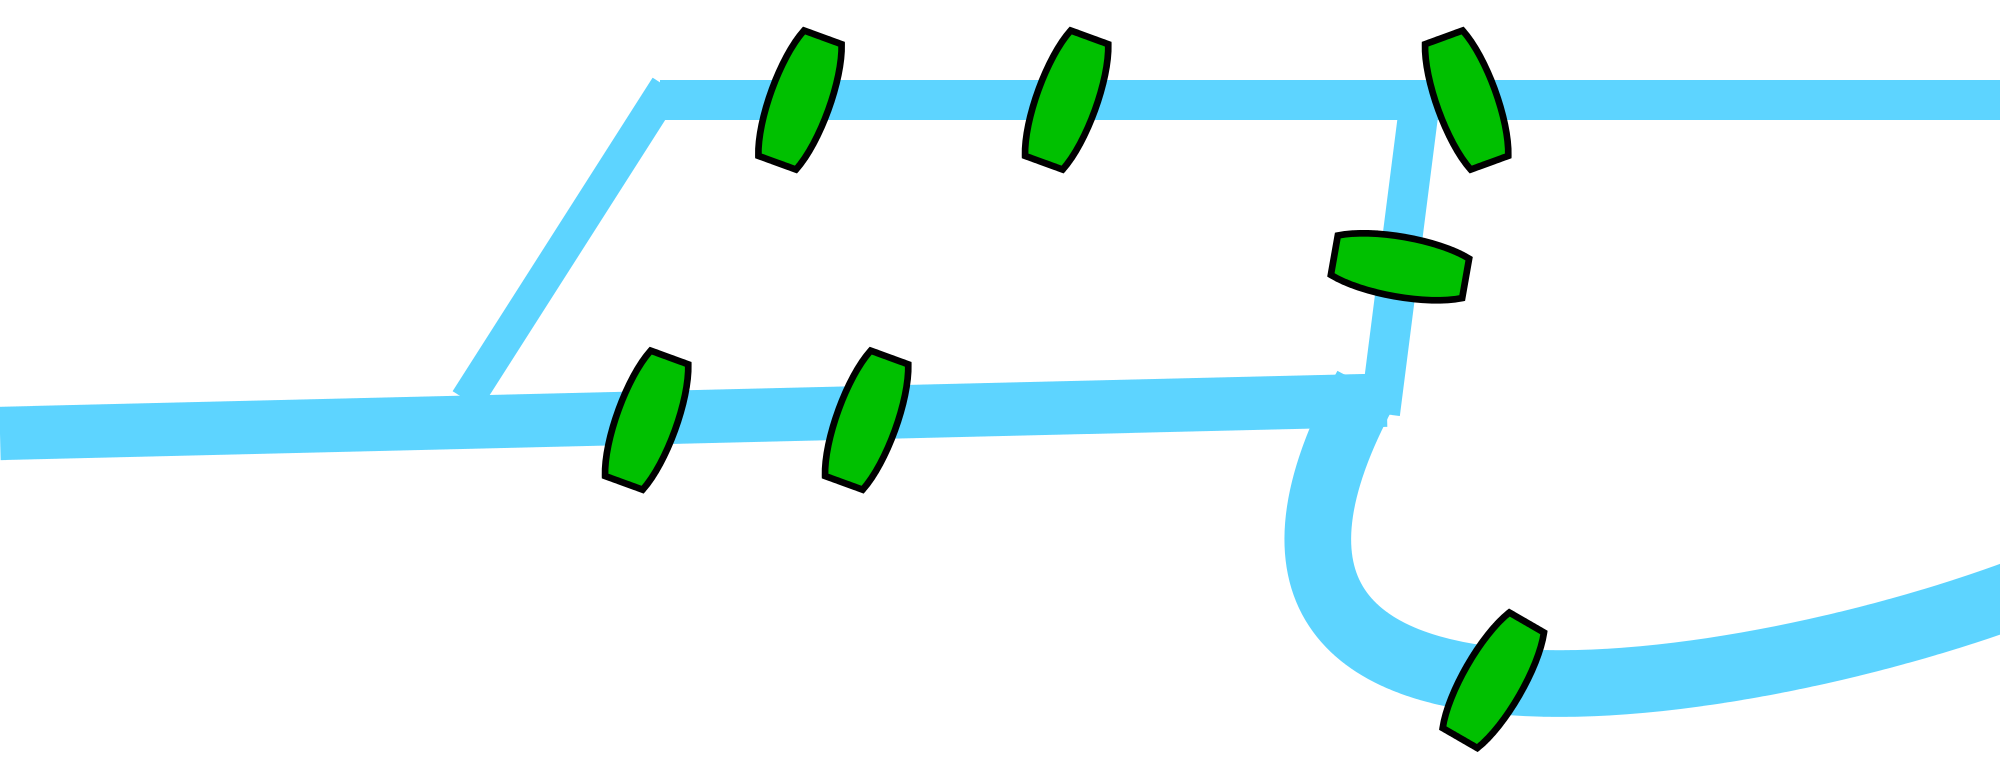
\includegraphics[width=10cm]{bridges.png} 
   \begin{center}
       \caption{\label{fig:my-label}Figure 1.1: Seven Bridges of K\"{o}nigsberg in Prussia}
   \end{center}
\end{center}


\indent This problem is also known as the “Seven Bridges of K\"{o}nigsberg” and is given a different approach by representing the four land masses in a form of a dot, and the bridges in a form of a line. These representations are collectively known as a graph. Graphs are made up of a collection of dots called vertices and lines connecting those dots called edges.\\

\indent A graph on $n$ vertices is said to be graceful if we can label all its vertices with integers from 0 to $n$, such that when an edge is labeled as the absolute difference of the numbers assigned to the vertices joining the edge, the edge will run from 1 to $n-1$.\\

\indent A tree is a connected simple graph without any cycles, or a tree is a connect acyclic graph. A tree on $n$ vertices is said to be graceful if its vertices can be labeled from 0 to $n-1$ such that the edge weights, that is equal to the absolute difference of the adjacent vertices, will run from 1 to $n-1$.\\

\indent In 1967, Gerhard Ringel and Anton Kotzig hypothesized that all trees are graceful. Up to this date,this conjecture has not yet proven, although some researches proved specific classes of trees. This problem lead to the discovery of new families of trees and some graceful labelling algorithms.
\section{Theoretical Background}
\indent
\indent To better understand problem, this section discusses the basic concepts, definitions, and lemmas about graphs, trees, and gracefulness of trees which will be used throughout the paper.

\begin{define} A graph $G$ is an ordered pair of $(V(G), (E(G)$, consisting of a non-empty set $V(G)$ of vertices and a set $E(G)$ of edges, disjoint from $V(G)$.
\end{define}
\indent 
\indent In a graph, the vertices are usually represented by dots, while edges are represented by curves or segments. For example, if $V(G)=$\{$v_0, v_1, v_2, v_3, v_4$\} and $E(G)=$\{$(v_0, v_1),(v_1, v_2), (v_2, v_2), (v_2, v_3), (v_3, v_4), (v_4, v_3), \\(v_4, v_0)$\}, then the graph may be presented as in Figure 2.1.
	\begin{center}
	\resizebox {0.4\textwidth} {0.9\height} {
		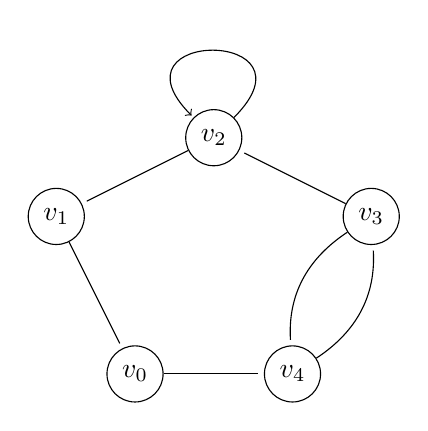
\begin{tikzpicture}[shorten >=2pt, auto, node distance=1cm,
		node_style/.style={circle,draw=black,fill=white!0!,font=\sffamily},
		edge_style/.style={draw=black}]
		
		\node[node_style] (n0) at (0,0)  {$v_0$};
		\node[node_style] (n4) at (2,0)  {$v_4$};
		\node[node_style] (n1) at (-1,2)  {$v_1$};
		\node[node_style] (n2) at (1,3)  {$v_2$};
		\node[node_style] (n3) at (3,2)  {$v_3$};
		
		\draw[edge_style]  (n0) edge node{} (n4);
    	\draw[edge_style]  (n4) edge[bend right] node{} (n3);
    	\draw[edge_style]  (n3) edge node{} (n2);
    	\draw[edge_style]  (n2) edge node{} (n1);
    	\draw[edge_style]  (n1) edge node{} (n0);
    	\draw[edge_style]  (n2) edge [loop] node{} (n2);
    	\draw[edge_style]  (n3) edge[bend right] node{} (n4);

    
		\end{tikzpicture}}
		\begin{center}
		    Figure 2.1
		\end{center}
\end{center}


\begin{define} If $a,b\in V(G)$ and $(a,b)\in E(G)$, $(a,b)$ is said to be incidents to both $a$ and $b$.
\end{define}

\begin{define} The \textbf{degree}, $d_G (v)$, of a vertex $v$ in a graph $G$ is the number of edges of $G$ incident with $u$, each loop counting as two edges.
\end{define}

\begin{define} A graph is \textbf{simple} if it has no loops and no two edges of its edges join the same pair of vertices.
\end{define}
\indent
\indent In Figure 2.1, since the graph contains a loop, the graph is not simple. Moreover, The graph has multiple edges.

\begin{define} A graph is \textbf{finite} if both its vertex set and edge set are finite.
\end{define}

\begin{define}
    A \textbf{walk} in a graph $G$ is a finite nonempty sequence $W=v_0 e_1 v_1 e_2 v_2 \dots e_k v_k$, whose terms are alternately vertices and edges of $G$, such that, for $1\leq i\leq k$, the ends of $e_i$ are $v_{i-1}$ and $v_i$. A walk is \textbf{closed} if its end and initial vertices are the same. If the vertices in a walk is distinct then the walk is called a \textbf{path}.
\end{define}

\begin{define} A graph is \textbf{cyclic} if it has a closed path. Otherwise, it is \textbf{acyclic}.
\end{define}

\begin{define} A graph $G$ is \textbf{connected} if there is a path between any two vertices in $G$.
\end{define}

\begin{define} A \textbf{tree} is an acyclic connected simple graph. 
\end{define}

\begin{define} A graph $G$ is \textbf{bipartite} if its vertex set can be partitioned into two nonempty subsets $A$ and $B$ such that each edge of $G$ has one end in $A$ and the other in $B$.
\end{define}
\indent
\indent A graph is bipartite if and only if it has no odd cycle. Since every tree is acyclic, then every tree is bipartite.


\begin{define} A \textbf{graceful numbering} or \textbf{valuation} of a graph $G$ with $m$ edges is an injection $g$ between the vertex set $V(G)$ of $G$ and $N_m^0=$\{$0,1,\dots,m$\} such that the induced function $w$ defined as $w(u,v)=|g(u)-g(v)|$ is a bijection between the edge set $E(G)$ and $N_m=$\{$1,2,\dots,m$\}.
\end{define}

\begin{define} A graph with a graceful numbering is called a \textbf{graceful graph}.
\end{define}

\begin{define} A tree $T$ with $n$ vertices has $n-1$ edges. Therefore, the graceful valuation of a tree $T$ is an injection between $V(T)$ and $N_{n-1}^0$ and which induces an injection between $E(T)$ and $N_{n-1}$.
\end{define}


\begin{define} The distance between two vertices in a tree $T$ is the length of the unique path joining them.
\end{define}

\begin{define} The \textbf{base} of a tree $T$ under a graceful valuation $g$ is the vertex $b$ in $T$ such that $g(b)=0$.
\end{define}

\begin{define} A graceful valuation $g$ of a tree $T$ is said to be \textbf{interlaced} if g induces, by restriction, a bijection between $P(b)$ and \{$0,1,2,\dots,{s-1}$\}, where $b$ is the base of $T$ under $g$, and, $s$ is the number of vertices of $T$ in $P(b)$ and the \textit{size} of $T$ under $g$.
\end{define}

The following lemmas are in Loyola's 1991 master's thesis.
\begin{lem} Let $T$ be a tree with $n$ vertices and a graceful valuation $g$. Suppose $g$ is interlaced and $s$ is the size of $T$ under $g$. Let $c$ and $d$ be non-negative integers and $g*$ be defined on $T$ by
\begin{center}
    $g^*(v)= $
    \begin{cases}
        $g(v)+c$, \text{if $v\in A_T$}\\
        $g(v)+d$, \text{if $v\in B_T$} 
    \end{cases}
    
\end{center}
Then, 
\begin{enumerate}
    \item[(a)]$g^*$ is an injection between $A_T$ and \{$c,c+1,\dots,s+c-1$\} 
    \item[(b)] $g^*$ is an injection between $B_T$ and \{$s+d, s+d+1,\dots, n+d-1$\}.
\end{enumerate}
\end{lem}

\begin{lem} Let $w$ be a one-to-one function induced by $g$ on $E(T)$ and $w^*$ be the function induced by $g^*$ on $E(T)$. Then, 

\begin{enumerate}
    \item[(a)] if $d\geq c$, $w^*$ is an injection between $E(T)$ and \{$d-c+1, d-c+2, \dots, d-c+n-1$\}.
    \item[(b)] if $c\geq d$, $w^*$ is an injection between $E(T)$ and \{$c-d-n+1,c-d-n+2, \dots, c-d-1$\}.
\end{enumerate}
\end{lem}

\begin{lem} Let $P=p_0 p_1 \dots p_{2n+5}$ be a path of length $2n+5$ where $n$ is even. Then, $P_{2n+6}$ has an interlaced valuation $h_1$ such that 
\begin{center}
      $h(p_{n+2})=\dfrac{3n+8}{2}$\\
      $h(p_{n+3})= \dfrac{3n+10}{2}$
\end{center}
and the size of $P_{2n+6}$ under $h_1$ is $n+3$.
\end{lem}

\begin{lem} Let $P=p_0 p_1 \dots p_{2n+5}$ be a path of length $2n+5$ where $n$ is odd. Then, $P_{2n+6}$ has an interlaced valuation $h_2$ such that 
\begin{center}
      $h(p_{n+2})=\dfrac{n+3}{2}$\\
      $h(p_{n+3})= \dfrac{n+1}{2}$
\end{center}
and the size of $P_{2n+6}$ under $h_2$ is $n+3$.
\end{lem}


\section{Review of Related Literature}
\indent
\indent In 1967, Gerhard Ringel and Anton Kotzig hypothesized that all trees are graceful. Up to this date,this conjecture has not yet proven. This problem lead to the discovery of new families of trees and some graceful labelling algorithms in the hope of proving or disproving this 50-year old conjecture.\\
\indent Here are some classes of graceful trees cited by Gallian in his book "A Dynamic Survey of Graph Labelling".
\begin{enumerate}
	\item \noindent {\bfseries Path}\\
	A path (or chain) is a walk with distinct vertices and edges. Shown in the figure below is a gracefully-labeled path on 7 vertices.\\

	\begin{center}
	\resizebox {0.5\textwidth} {0.5\height} {
		
		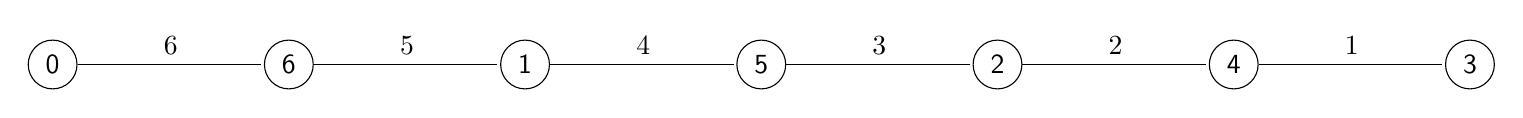
\begin{tikzpicture}[shorten >=1pt, auto, node distance=3cm,
		node_style/.style={circle,draw=black,fill=white!20!,font=\sffamily},
		edge_style/.style={draw=black}]
		\node[node_style] (n0) at (4,9)  {0};
		\node[node_style] (n6) at (7,9) {6};
		\node[node_style] (n1) at (10,9)  {1};
		\node[node_style] (n5) at (13,9)  {5};
		\node[node_style] (n2) at (16,9) {2};
		\node[node_style] (n4) at (19,9)  {4};
		\node[node_style] (n3) at (22,9)  {3};
		\draw[edge_style]  (n0) edge node{6} (n6);
		\draw[edge_style]  (n6) edge node{5} (n1);
		\draw[edge_style]  (n1) edge node{4} (n5);
		\draw[edge_style]  (n5) edge node{3} (n2);
		\draw[edge_style]  (n2) edge node{2} (n4);
		\draw[edge_style]  (n4) edge node{1} (n3);
		\end{tikzpicture}}
\end{center}
		



	\item \noindent {\bfseries Caterpillars}\\
	A caterpillar is a tree where the removal of its vertices of degree one leaves a path. Shown in the figure below is a gracefully-labeled caterpillar on 14 vertices.\\
	\begin{center}
		\resizebox {0.6\textwidth} {0.5\height} {
			\begin{tikzpicture}[shorten >=1pt, auto, node distance=3cm,
			node_style/.style={circle,draw=black,fill=white!20!,font=\sffamily},
			edge_style/.style={draw=black}]
			\node[node_style] (n12) at (7,11)  {12};
			\node[node_style] (n9) at (13,11) {9};
			\node[node_style] (n5) at (16,11)  {5};
			\node[node_style] (n13) at (3,9)  {13};
			\node[node_style] (n2) at (7,9) {2};
			\node[node_style] (n10) at (10,9)  {10};
			\node[node_style] (n4) at (13,9)  {4};
			\node[node_style] (n8) at (16,9)  {8};
			\node[node_style] (n6) at (19,9) {6};
			\node[node_style] (n0) at (1,7)  {0};
			\node[node_style] (n1) at (4,7)  {1};
			\node[node_style] (n11) at (7,7) {11};
			\node[node_style] (n3) at (10,7)  {3};
			\node[node_style] (n7) at (16,7)  {7};
			\draw[edge_style]  (n0) edge node{13} (n13);
			\draw[edge_style]  (n1) edge node{12} (n13);
			\draw[edge_style]  (n2) edge node{11} (n13);
			\draw[edge_style]  (n2) edge node{9} (n11);
			\draw[edge_style]  (n2) edge node{10} (n12);
			\draw[edge_style]  (n2) edge node{8} (n10);
			\draw[edge_style]  (n3) edge node{7} (n10);
			\draw[edge_style]  (n4) edge node{6} (n10);
			\draw[edge_style]  (n4) edge node{5} (n9);
			\draw[edge_style]  (n4) edge node{4} (n8);
			\draw[edge_style]  (n5) edge node{3} (n8);
			\draw[edge_style]  (n7) edge node{1} (n8);
			\draw[edge_style]  (n8) edge node{2} (n6);
			\end{tikzpicture}}
\end{center}	

	\item \noindent {\bfseries Symmetrical Trees}\\
A symmetrical tree is a rooted tree in which every level contains vertices of the same degree. Shown in the figure below is a gracefully-labeled symmetrical tree on 11 vertices.\\
\begin{center}
	\resizebox {0.3\textwidth} {0.5\height} {
		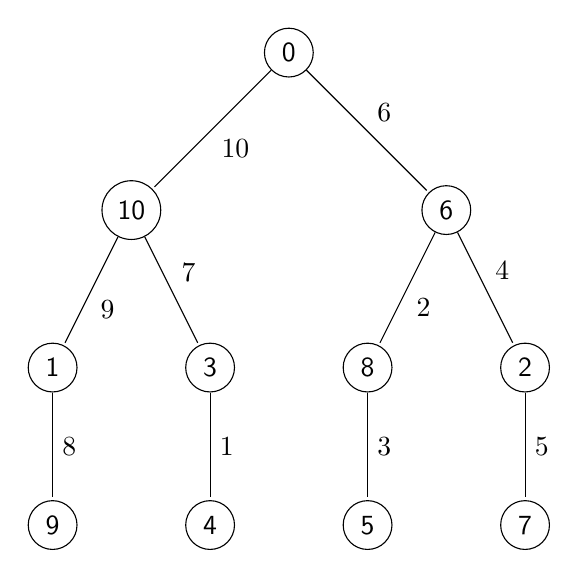
\begin{tikzpicture}[shorten >=1pt, auto, node distance=3cm,
		node_style/.style={circle,draw=black,fill=white!20!,font=\sffamily},
		edge_style/.style={draw=black}]
		\node[node_style] (n0) at (5,13)  {0};
		\node[node_style] (n10) at (3,11) {10};
		\node[node_style] (n6) at (7,11)  {6};
		\node[node_style] (n1) at (2,9) {1};
		\node[node_style] (n3) at (4,9)  {3};
		\node[node_style] (n8) at (6,9)  {8};
		\node[node_style] (n2) at (8,9)  {2};
		\node[node_style] (n9) at (2,7) {9};
		\node[node_style] (n4) at (4,7)  {4};
		\node[node_style] (n5) at (6,7)  {5};
		\node[node_style] (n7) at (8,7)  {7};
		\draw[edge_style]  (n0) edge node{10} (n10);
		\draw[edge_style]  (n0) edge node{6} (n6);
		\draw[edge_style]  (n10) edge node{9} (n1);
		\draw[edge_style]  (n10) edge node{7} (n3);
		\draw[edge_style]  (n6) edge node{2} (n8);
		\draw[edge_style]  (n6) edge node{4} (n2);
		\draw[edge_style]  (n1) edge node{8} (n9);
		\draw[edge_style]  (n3) edge node{1} (n4);
		\draw[edge_style]  (n8) edge node{3} (n5);
		\draw[edge_style]  (n2) edge node{5} (n7);
		\end{tikzpicture}}
\end{center}	


\item {\bfseries Olive Trees}\\
    An Olive tree is formed by attaching paths of consecutive lengths in a single vertex. Shown below is an example of a graceful olive tree.
	\begin{center}
	\resizebox {0.3\textwidth} {0.7\height} {
		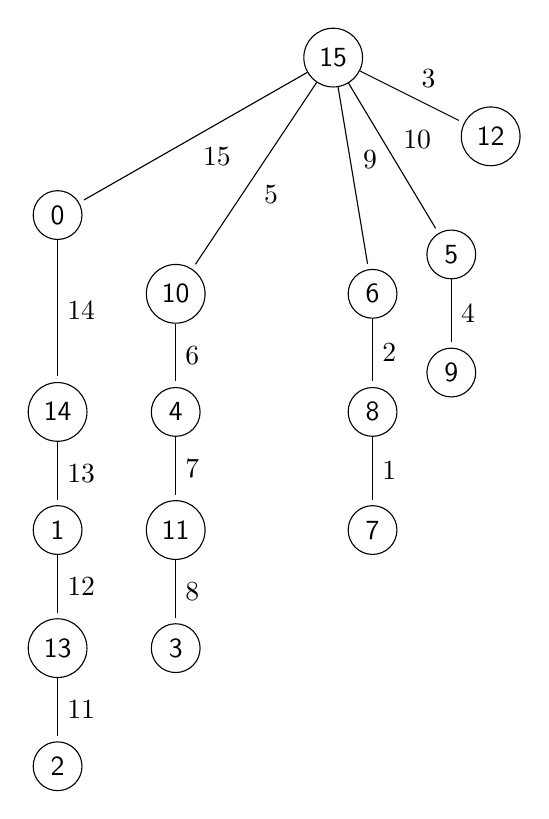
\begin{tikzpicture}[shorten >=2pt, auto, node distance=1cm,
		node_style/.style={circle,draw=black,fill=white!0!,font=\sffamily},
		edge_style/.style={draw=black}]
		
		\node[node_style] (n15) at (3,3)  {15};
		\node[node_style] (n12) at (5,2)  {12};
		\node[node_style] (n5) at (4.5,0.5)  {5};
		\node[node_style] (n9) at (4.5,-1)  {9};
		\node[node_style] (n6) at (3.5,0)  {6};
		\node[node_style] (n8) at (3.5,-1.5)  {8};
		\node[node_style] (n7) at (3.5,-3)  {7};
		\node[node_style] (n10) at (1,0)  {10};
		\node[node_style] (n4) at (1,-1.5)  {4};
		\node[node_style] (n11) at (1,-3)  {11};
		\node[node_style] (n3) at (1,-4.5)  {3};
		\node[node_style] (n0) at (-0.5,1)  {0};
		\node[node_style] (n14) at (-0.5,-1.5)  {14};
		\node[node_style] (n1) at (-0.5,-3)  {1};
	    \node[node_style] (n13) at (-0.5,-4.5)  {13};
		\node[node_style] (n2) at (-0.5,-6)  {2};
		
		\draw[edge_style]  (n15) edge node{3} (n12);
    	\draw[edge_style]  (n15) edge node{10} (n5);
    	\draw[edge_style]  (n5) edge node{4} (n9);
    	\draw[edge_style]  (n15) edge node{9} (n6);
    	\draw[edge_style]  (n6) edge node{2} (n8);
    	\draw[edge_style]  (n8) edge node{1} (n7);
    	\draw[edge_style]  (n15) edge node{5} (n10);
    	\draw[edge_style]  (n10) edge node{6} (n4);
    	\draw[edge_style]  (n4) edge node{7} (n11);
    	\draw[edge_style]  (n11) edge node{8} (n3);
    	\draw[edge_style]  (n15) edge node{15} (n0);
    	\draw[edge_style]  (n0) edge node{14} (n14);
    	\draw[edge_style]  (n14) edge node{13} (n1);
    	\draw[edge_style]  (n1) edge node{12} (n13);
    	\draw[edge_style]  (n13) edge node{11} (n2);
    
		\end{tikzpicture}}

		
\end{center}

    Dr. Jean Loyola \cite{Loyola} discovered three new families of graceful trees.
%12	
\item {\bfseries $J_n$ Trees}\\
    $J_n$ trees are constructed by planting an end vertex of a path of length $i$, for $i=0,1,2,...,n-1$, in a parent path $v_0 v_1 v_2...v_{n-1}$ with a length of $n-1$. Shown below is an example of a graceful $J_4$ tree.
    \\

	\begin{center}
	\resizebox {0.3\textwidth} {0.7\height} {
		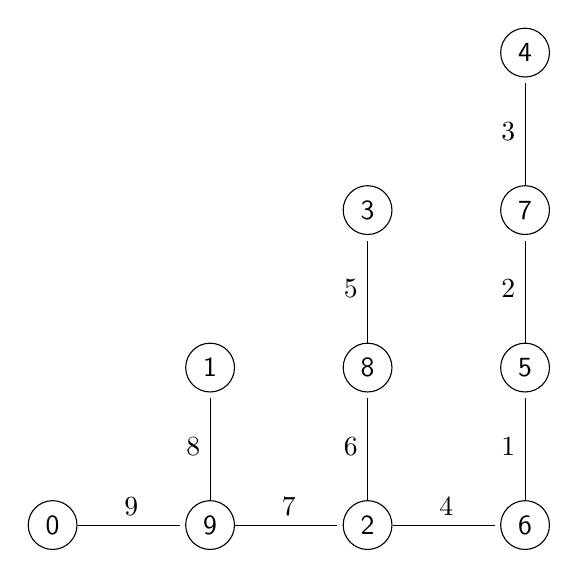
\begin{tikzpicture}[shorten >=2pt, auto, node distance=1cm,
		node_style/.style={circle,draw=black,fill=white!0!,font=\sffamily},
		edge_style/.style={draw=black}]
		
		\node[node_style] (n0) at (0,0)  {0};
		\node[node_style] (n9) at (2,0)  {9};
		\node[node_style] (n2) at (4,0)  {2};
		\node[node_style] (n6) at (6,0)  {6};
		\node[node_style] (n1) at (2,2)  {1};
		\node[node_style] (n8) at (4,2)  {8};
		\node[node_style] (n3) at (4,4)  {3};
		\node[node_style] (n5) at (6,2)  {5};
		\node[node_style] (n7) at (6,4)  {7};
		\node[node_style] (n4) at (6,6)  {4};
		
		
		\draw[edge_style]  (n0) edge node{9} (n9);
    	\draw[edge_style]  (n9) edge node{7} (n2);
    	\draw[edge_style]  (n2) edge node{4} (n6);
    	\draw[edge_style]  (n9) edge node{8} (n1);
    	\draw[edge_style]  (n2) edge node{6} (n8);
    	\draw[edge_style]  (n8) edge node{5} (n3);
    	\draw[edge_style]  (n6) edge node{1} (n5);
    	\draw[edge_style]  (n5) edge node{2} (n7);
    	\draw[edge_style]  (n7) edge node{3} (n4);
		\end{tikzpicture}}
		
	
		
\end{center}
%13	
\item {\bfseries $J_{n,m}$ Trees}\\
    % NEEDS DEFINITION
    A $J_{n,m}$ tree is formed by taking $m$ copies of the $J_n$ tree and making the classification $v_{0,i}=v_{0,j}$ for all $0 {\geq} i$, $j {\geq} m$, provided that $m,n {\geq} 2$.Shown below is an example of a graceful $J_{3,3}$ tree.
	\\
	\begin{center}
	\resizebox {0.5\textwidth} {0.7\height} {
		\begin{tikzpicture}[shorten >=2pt, auto, node distance=1cm,
		node_style/.style={circle,draw=black,fill=white!0!,font=\sffamily},
		edge_style/.style={draw=black}]
		
		\node[node_style] (n0) at (3,0)  {0};
		\node[node_style] (n15) at (5,1)  {15};
		\node[node_style] (n10) at (1,1)  {10};
		\node[node_style] (n5) at (3,-2)  {5};
		\node[node_style] (n12) at (3,-4)  {12};
		\node[node_style] (n11) at (1,-2)  {11};
		\node[node_style] (n4) at (1,-4)  {4};
		\node[node_style] (n13) at (-1,-4)  {5};
		\node[node_style] (n7) at (-1,2)  {7};
		\node[node_style] (n6) at (3,2)  {6};
		\node[node_style] (n1) at (7,0)  {1};
		\node[node_style] (n2) at (7,2)  {2};
		\node[node_style] (n14) at (9,1)  {14};
		\node[node_style] (n3) at (11,0)  {3};
		\node[node_style] (n9) at (1,3)  {9};
		\node[node_style] (n8) at (3,4)  {8};
		
		\draw[edge_style]  (n0) edge node{10} (n10);
    	\draw[edge_style]  (n10) edge node{3} (n7);
    	\draw[edge_style]  (n7) edge node{2} (n9);
    	\draw[edge_style]  (n9) edge node{1} (n8);
    	\draw[edge_style]  (n10) edge node{4} (n6);
    	\draw[edge_style]  (n0) edge node{15} (n15);
    	\draw[edge_style]  (n15) edge node{14} (n1);
    	\draw[edge_style]  (n15) edge node{13} (n2);
    	\draw[edge_style]  (n2) edge node{12} (n14);
        \draw[edge_style]  (n14) edge node{11} (n3);
        \draw[edge_style]  (n0) edge node{5} (n5);
    	\draw[edge_style]  (n5) edge node{6} (n11);
    	\draw[edge_style]  (n5) edge node{7} (n12);
    	\draw[edge_style]  (n12) edge node{8} (n4);
        \draw[edge_style]  (n13) edge node{9} (n4);
    
		\end{tikzpicture}}
		
		
		
\end{center}

%14
\item {\bfseries $J_n$ + $J_{n+1}$ Trees}\\
    % NEEDS DEFINITION
    \indent 
    A  $J_n$ + $J_{n+1}$ tree is formed considering  $J_n$ and $J_{n+1}$ and making the identification
   
    $v_{i,n}=v_{i+n,n+1}$ for all $1\leq i\leq n-1$.Shown below is an example of a graceful $J_2$ + $J_3$ tree.
	\\
	\begin{center}
	\resizebox {0.3\textwidth} {0.7\height} {
		\begin{tikzpicture}[shorten >=2pt, auto, node distance=1cm,
		node_style/.style={circle,draw=black,fill=white!0!,font=\sffamily},
		edge_style/.style={draw=black}]
		
		\node[node_style] (n5) at (0,0)  {5};
		\node[node_style] (n2) at (2,0)  {2};
		\node[node_style] (n4) at (4,0)  {4};
		\node[node_style] (n3) at (6,0)  {3};
		\node[node_style] (n6) at (2,2)  {6};
		\node[node_style] (n0) at (2,4)  {0};
		\node[node_style] (n1) at (4,2)  {1};
	
		
		\draw[edge_style]  (n5) edge node{3} (n2);
    	\draw[edge_style]  (n2) edge node{2} (n4);
    	\draw[edge_style]  (n4) edge node{1} (n3);
    	\draw[edge_style]  (n2) edge node{4} (n6);
    	\draw[edge_style]  (n0) edge node{6} (n6);
    	\draw[edge_style]  (n6) edge node{5} (n1);
    
    
		\end{tikzpicture}}
		
		
\end{center}

%15

Castilan and Zarraga \cite{Castilan and Zarraga} discover three new familes of graceful trees namely, $\overline{P}_{(0,1)_n}(f)$,  $\overline{P}_{(0,2)_n}(f)$, and  $\overline{P}_{(0,3)_n}(f)$
\item {\bfseries $\overline{P}_{(0,1)_n}(f)$ Trees}\\
    % NEEDS DEFINITION
    Let $f(i)=k$ if $n=2k-1$ or $n=2k$. Let  $\overline{P}_{(0,1)_n}(f)=v_0 v_1 v_2\dots v_n$ be a path of length $n$ where $n$ is an even integer. Let $\overline{P}_{(0,1)_n}(f)$ be the tree obtained by planting an end vertex of a path $\overline{P}_i$ of length $f(i)$ to each $v_i$ for $i=1,2,\dots,n$. Shown below is an example of a graceful $\overline{P}_{(0,1)_4}(f)$ tree.
	\\
	\begin{center}
	\resizebox {0.4\textwidth} {0.7\height} {
		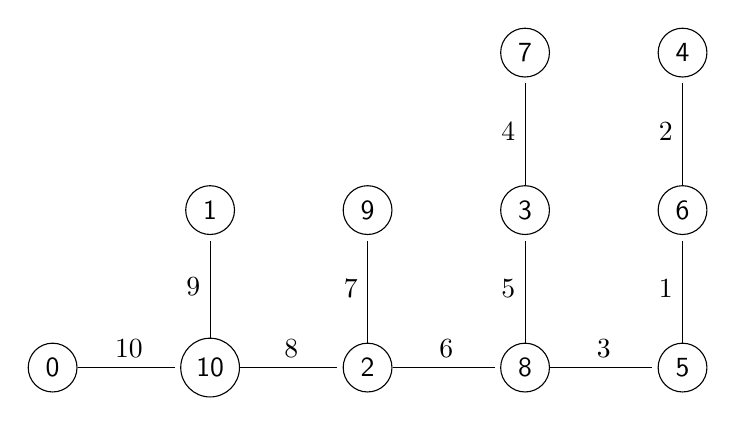
\begin{tikzpicture}[shorten >=2pt, auto, node distance=1cm,
		node_style/.style={circle,draw=black,fill=white!0!,font=\sffamily},
		edge_style/.style={draw=black}]
		
		\node[node_style] (n0) at (0,0)  {0};
		\node[node_style] (n10) at (2,0)  {10};
		\node[node_style] (n1) at (2,2)  {1};
		\node[node_style] (n2) at (4,0)  {2};
		\node[node_style] (n9) at (4,2)  {9};
		\node[node_style] (n8) at (6,0)  {8};
		\node[node_style] (n3) at (6,2)  {3};
	    \node[node_style] (n7) at (6,4)  {7};
		\node[node_style] (n5) at (8,0)  {5};
		\node[node_style] (n6) at (8,2)  {6};
		\node[node_style] (n4) at (8,4)  {4};
		
		\draw[edge_style]  (n0) edge node{10} (n10);
    	\draw[edge_style]  (n10) edge node{9} (n1);
    	\draw[edge_style]  (n10) edge node{8} (n2);
    	\draw[edge_style]  (n2) edge node{7} (n9);
    	\draw[edge_style]  (n2) edge node{6} (n8);
    	\draw[edge_style]  (n8) edge node{3} (n5);
        \draw[edge_style]  (n8) edge node{5} (n3);
    	\draw[edge_style]  (n3) edge node{4} (n7);
    	\draw[edge_style]  (n5) edge node{1} (n6);
    	\draw[edge_style]  (n6) edge node{2} (n4);
    
		\end{tikzpicture}}

\end{center}
\item {\bfseries $\overline{P}_{(0,2)_n}(f)$ Trees}\\
    % NEEDS DEFINITION
    Let $f(i)=k+1$ if $n=2k-1$ or $n=2k$. Let  $\overline{P}_{(0,2)_n}(f)=v_0 v_1 v_2\dots v_n$ be a path of length $n$ where $n$ is an even integer. Let $\overline{P}_{(0,2)_n}(f)$ be the tree obtained by planting an end vertex of a path $\overline{P}_i$ of length $f(i)$ to each $v_i$ for $i=1,2,\dots,n$. Shown below is an example of a graceful $\overline{P}_{(0,2)_4}(f)$ tree.
	\\
	\begin{center}
	\resizebox {0.4\textwidth} {0.7\height} {
		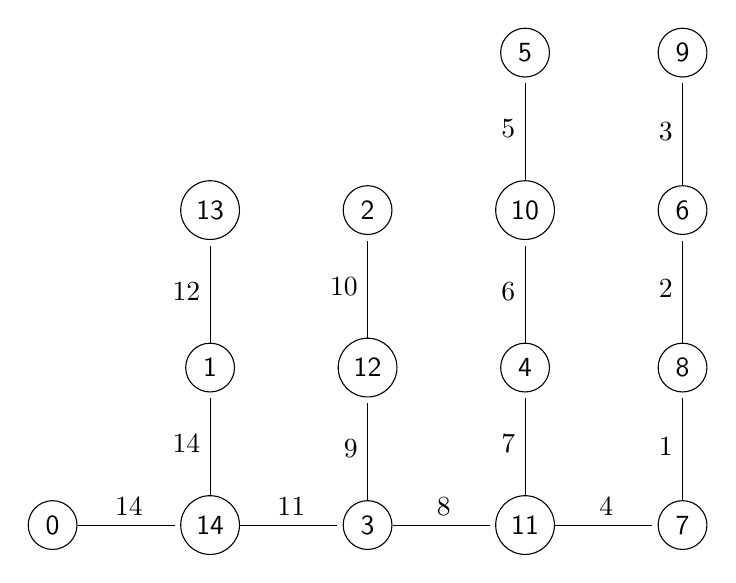
\begin{tikzpicture}[shorten >=2pt, auto, node distance=1cm,
		node_style/.style={circle,draw=black,fill=white!0!,font=\sffamily},
		edge_style/.style={draw=black}]
		
		\node[node_style] (n0) at (0,0)  {0};
		\node[node_style] (n14) at (2,0)  {14};
		\node[node_style] (n1) at (2,2)  {1};
		\node[node_style] (n13) at (2,4)  {13};
		\node[node_style] (n3) at (4,0)  {3};
		\node[node_style] (n12) at (4,2)  {12};
		\node[node_style] (n2) at (4,4)  {2};
	    \node[node_style] (n11) at (6,0)  {11};
		\node[node_style] (n4) at (6,2)  {4};
		\node[node_style] (n10) at (6,4)  {10};
		\node[node_style] (n5) at (6,6)  {5};
	    \node[node_style] (n7) at (8,0)  {7};
		\node[node_style] (n8) at (8,2)  {8};
		\node[node_style] (n6) at (8,4)  {6};
		\node[node_style] (n9) at (8,6)  {9};
		
		\draw[edge_style]  (n0) edge node{14} (n14);
    	\draw[edge_style]  (n14) edge node{14} (n1);
    	\draw[edge_style]  (n1) edge node{12} (n13);
    	\draw[edge_style]  (n14) edge node{11} (n3);
    	\draw[edge_style]  (n3) edge node{9} (n12);
    	\draw[edge_style]  (n12) edge node{10} (n2);
        \draw[edge_style]  (n3) edge node{8} (n11);
    	\draw[edge_style]  (n11) edge node{7} (n4);
    	\draw[edge_style]  (n4) edge node{6} (n10);
    	\draw[edge_style]  (n10) edge node{5} (n5);
        \draw[edge_style]  (n11) edge node{4} (n7);
    	\draw[edge_style]  (n7) edge node{1} (n8);
    	\draw[edge_style]  (n8) edge node{2} (n6);
    	\draw[edge_style]  (n6) edge node{3} (n9);
    
		\end{tikzpicture}}

\end{center}

\item {\bfseries $\overline{P}_{(0,3)_n}$ $(f)$ Trees}\\
    % NEEDS DEFINITION
     Let $f(i)=k+2$ if $n=2k-1$ or $n=2k$, $k\geq1$. Let $\overline{P}_{(0,3)_n}(f)=v_0 v_1 v_2\dots v_n$ be a path of length $n$ where $n$ is an even integer. Let $\overline{P}_{(0,3)_n}(f)$ be the tree obtained by planting an end vertex of a path $\overline{P}_i$ of length $f(i)$ to each $v_i$ for $i=1,2,\dots,n$.Shown below is an example of a graceful $\overline{P}_{(0,3)_4}(f)$ tree.
	\\
	\begin{center}
	\resizebox {0.4\textwidth} {0.7\height} {
		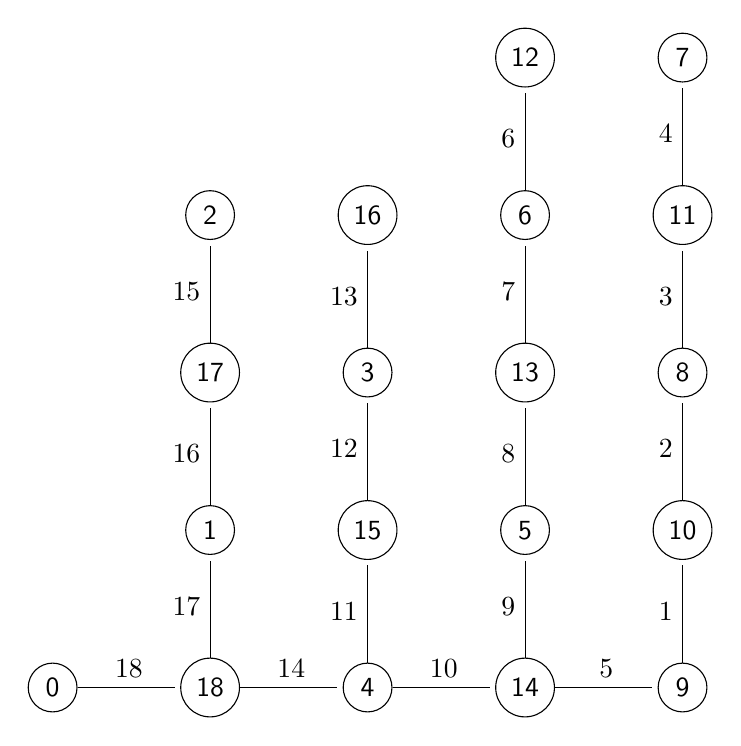
\begin{tikzpicture}[shorten >=2pt, auto, node distance=1cm,
		node_style/.style={circle,draw=black,fill=white!0!,font=\sffamily},
		edge_style/.style={draw=black}]
		
		\node[node_style] (n0) at (0,0)  {0};
		\node[node_style] (n18) at (2,0)  {18};
		\node[node_style] (n1) at (2,2)  {1};
		\node[node_style] (n17) at (2,4)  {17};
		\node[node_style] (n2) at (2,6)  {2};
		\node[node_style] (n4) at (4,0)  {4};
		\node[node_style] (n15) at (4,2)  {15};
	    \node[node_style] (n3) at (4,4)  {3};
		\node[node_style] (n16) at (4,6)  {16};
		\node[node_style] (n14) at (6,0)  {14};
		\node[node_style] (n5) at (6,2)  {5};
		\node[node_style] (n13) at (6,4)  {13};
		\node[node_style] (n6) at (6,6)  {6};
		\node[node_style] (n12) at (6,8)  {12};
		\node[node_style] (n9) at (8,0)  {9};
		\node[node_style] (n10) at (8,2)  {10};
		\node[node_style] (n8) at (8,4)  {8};
		\node[node_style] (n11) at (8,6)  {11};
		\node[node_style] (n7) at (8,8)  {7};
		
		
		\draw[edge_style]  (n0) edge node{18} (n18);
    	\draw[edge_style]  (n18) edge node{17} (n1);
    	\draw[edge_style]  (n1) edge node{16} (n17);
    	\draw[edge_style]  (n17) edge node{15} (n2);
    	\draw[edge_style]  (n18) edge node{14} (n4);
    	\draw[edge_style]  (n4) edge node{11} (n15);
        \draw[edge_style]  (n15) edge node{12} (n3);
    	\draw[edge_style]  (n3) edge node{13} (n16);
    	\draw[edge_style]  (n4) edge node{10} (n14);
    	\draw[edge_style]  (n14) edge node{9} (n5);
    	\draw[edge_style]  (n5) edge node{8} (n13);
    	\draw[edge_style]  (n13) edge node{7} (n6);
    	\draw[edge_style]  (n6) edge node{6} (n12);
    	\draw[edge_style]  (n14) edge node{5} (n9);
    	\draw[edge_style]  (n9) edge node{1} (n10);
    	\draw[edge_style]  (n10) edge node{2} (n8);
    	\draw[edge_style]  (n8) edge node{3} (n11);
    	\draw[edge_style]  (n11) edge node{4} (n7);
    
		\end{tikzpicture}}
\end{center}


\end{enumerate}

\section{Objectives}

\noindent This seminar aims:
\begin{itemize}
	\item[a.] to present the collection and illustrations of known families of graceful trees;
	\item[b.] to discuss the new addition to the collection of families of graceful trees; and 
	\item[c.] to illustrate the the interlaced graceful valuation of each member of the families identified.
\end{itemize}

\section{Results}
\indent
\indent In this chapter, we introduce a new family of graceful trees by providing an interlaced valuation of each member of the family. \\
\indent Let $F_1 (2)$ be the tree formed by considering a $J_2$ tree with a parent path $P_2=v_0 v_1 $ and by planting a path $\overline{P}_2$ of length two to vertex  $v_1$. 
	\begin{center}
	\resizebox {0.15\textwidth} {0.7\height} {
		\begin{tikzpicture}[shorten >=2pt, auto, node distance=1cm,
		node_style/.style={circle,draw=black,fill=white!0!,font=\sffamily},
		edge_style/.style={draw=black}]
		
		\node[node_style] (n0) at (0,0)  {$v_0$};
		\node[node_style] (n1) at (2,0)  {$v_1$};
		\node[node_style] (n2) at (2,2)  {};
		\node[node_style] (n3) at (2,-2)  {};
		\node[node_style] (n4) at (2,-4)  {};
		
		\draw[edge_style]  (n0) edge node{} (n1);
    	\draw[edge_style]  (n1) edge node{} (n2);
    	\draw[edge_style]  (n1) edge node{} (n3);
    	\draw[edge_style]  (n3) edge node{} (n4);
    
		\end{tikzpicture}}\\
		\begin{center}
        $J_2$ tree with attached path of length 2 to vertex $v_1$.
    \end{center}
\end{center}
\indent For $n=2$, $F_2 (2)$ is formed by considering the $J_3$ tree with a parent path $P_3=v_0 v_1 v_2 $ and by planting a path $\overline{P}_2$ of length two to vertices $v_1$ and $v_2$. 
	\begin{center}
	\resizebox {0.25\textwidth} {0.7\height} {
		\begin{tikzpicture}[shorten >=2pt, auto, node distance=1cm,
		node_style/.style={circle,draw=black,fill=white!0!,font=\sffamily},
		edge_style/.style={draw=black}]
		
		\node[node_style] (n0) at (0,0)  {$v_0$};
		\node[node_style] (n1) at (2,0)  {$v_1$};
		\node[node_style] (n2) at (4,0)  {$v_2$};
		\node[node_style] (n3) at (2,2)  {};
		\node[node_style] (n4) at (4,2)  {};
		\node[node_style] (n5) at (4,4)  {};
	    \node[node_style] (n6) at (2,-2)  {};
		\node[node_style] (n7) at (4,-2)  {};
		\node[node_style] (n8) at (2,-4)  {};
		\node[node_style] (n9) at (4,-4)  {};
		
		\draw[edge_style]  (n0) edge node{} (n1);
    	\draw[edge_style]  (n1) edge node{} (n2);
    	\draw[edge_style]  (n1) edge node{} (n3);
    	\draw[edge_style]  (n2) edge node{} (n4);
    	\draw[edge_style]  (n4) edge node{} (n5);
    	\draw[edge_style]  (n1) edge node{} (n6);
    	\draw[edge_style]  (n2) edge node{} (n7);
    	\draw[edge_style]  (n6) edge node{} (n8);
    	\draw[edge_style]  (n7) edge node{} (n9);
    
		\end{tikzpicture}}\\
		\begin{center}
        $J_3$ tree with attached path of length 2 to vertices $v_1$ and $v_2$.
    \end{center}
\end{center}
\newpage
\indent
\indent For $n=3$, $F_3 (2)$ is formed by considering the $J_4$ tree with a parent path $P_4=v_0 v_1 v_2 v_3$ and by planting a path $\overline{P}_2$ of length two to vertices $v_1$, $v_2$, and $v_3$. 
\begin{center}
	\resizebox {0.35\textwidth} {0.7\height} {
		\begin{tikzpicture}[shorten >=2pt, auto, node distance=1cm,
		node_style/.style={circle,draw=black,fill=white!0!,font=\sffamily},
		edge_style/.style={draw=black}]
		
		\node[node_style] (n0) at (0,0)  {$v_0$};
		\node[node_style] (n1) at (2,0)  {$v_1$};
		\node[node_style] (n2) at (4,0)  {$v_2$};
		\node[node_style] (n3) at (6,0)  {$v_3$};
		\node[node_style] (n4) at (2,2)  {};
		\node[node_style] (n5) at (4,2)  {};
	    \node[node_style] (n6) at (4,4)  {};
		\node[node_style] (n7) at (6,2)  {};
		\node[node_style] (n8) at (6,4)  {};
		\node[node_style] (n9) at (6,6)  {};
		\node[node_style] (n10) at (2,-2)  {};
		\node[node_style] (n11) at (2,-4)  {};
	    \node[node_style] (n12) at (4,-2)  {};
		\node[node_style] (n13) at (4,-4)  {};
		\node[node_style] (n14) at (6,-2)  {};
		\node[node_style] (n15) at (6,-4)  {};
		
		\draw[edge_style]  (n0) edge node{} (n1);
    	\draw[edge_style]  (n1) edge node{} (n2);
    	\draw[edge_style]  (n2) edge node{} (n3);
    	\draw[edge_style]  (n1) edge node{} (n4);
    	\draw[edge_style]  (n2) edge node{} (n5);
    	\draw[edge_style]  (n5) edge node{} (n6);
    	\draw[edge_style]  (n3) edge node{} (n7);
    	\draw[edge_style]  (n7) edge node{} (n8);
    	\draw[edge_style]  (n8) edge node{} (n9);
    	\draw[edge_style]  (n1) edge node{} (n10);
    	\draw[edge_style]  (n10) edge node{} (n11);
    	\draw[edge_style]  (n2) edge node{} (n12);
    	\draw[edge_style]  (n12) edge node{} (n13);
    	\draw[edge_style]  (n3) edge node{} (n14);
    	\draw[edge_style]  (n14) edge node{} (n15);
    	
		\end{tikzpicture}}\\
		\begin{center}
        $J_4$ tree with attached path of length 2 to vertices $v_1$, $v_2$, and $v_3$.
    \end{center}
\end{center}
\indent
\indent For $n=4$, $F_4 (2)$ is formed by considering the $J_5$ tree with a parent path $P_5=v_0 v_1 v_2 v_3 v_4$ and by planting a path $\overline{P}_2$ of length two to vertices $v_1$, $v_2$, $v_3$ and $v_4$. 
\begin{center}
	\resizebox {0.45\textwidth} {0.7\height} {
		\begin{tikzpicture}[shorten >=2pt, auto, node distance=1cm,
		node_style/.style={circle,draw=black,fill=white!0!,font=\sffamily},
		edge_style/.style={draw=black}]
		
		\node[node_style] (n0) at (0,0)  {$v_0$};
		\node[node_style] (n1) at (2,0)  {$v_1$};
		\node[node_style] (n2) at (4,0)  {$v_2$};
		\node[node_style] (n3) at (6,0)  {$v_3$};
		\node[node_style] (n4) at (8,0)  {$v_4$};
		\node[node_style] (n5) at (2,2)  {};
	    \node[node_style] (n6) at (4,2)  {};
		\node[node_style] (n7) at (4,4)  {};
		\node[node_style] (n8) at (6,2)  {};
		\node[node_style] (n9) at (6,4)  {};
		\node[node_style] (n10) at (6,6)  {};
		\node[node_style] (n11) at (8,2)  {};
	    \node[node_style] (n12) at (8,4)  {};
		\node[node_style] (n13) at (8,6)  {};
		\node[node_style] (n14) at (8,8)  {};
		\node[node_style] (n15) at (2,-2)  {};
		\node[node_style] (n16) at (2,-4)  {};
		\node[node_style] (n17) at (4,-2)  {};
		\node[node_style] (n18) at (4,-4)  {};
		\node[node_style] (n19) at (6,-2)  {};
	    \node[node_style] (n20) at (6,-4)  {};
		\node[node_style] (n21) at (8,-2)  {};
		\node[node_style] (n22) at (8,-4)  {};

		\draw[edge_style]  (n0) edge node{} (n1);
    	\draw[edge_style]  (n1) edge node{} (n2);
    	\draw[edge_style]  (n2) edge node{} (n3);
    	\draw[edge_style]  (n3) edge node{} (n4);
    	\draw[edge_style]  (n1) edge node{} (n5);
    	\draw[edge_style]  (n2) edge node{} (n6);
    	\draw[edge_style]  (n6) edge node{} (n7);
    	\draw[edge_style]  (n3) edge node{} (n8);
    	\draw[edge_style]  (n8) edge node{} (n9);
    	\draw[edge_style]  (n9) edge node{} (n10);
    	\draw[edge_style]  (n4) edge node{} (n11);
    	\draw[edge_style]  (n11) edge node{} (n12);
    	\draw[edge_style]  (n12) edge node{} (n13);
    	\draw[edge_style]  (n13) edge node{} (n14);
    	\draw[edge_style]  (n1) edge node{} (n15);
    	\draw[edge_style]  (n15) edge node{} (n16);
    	\draw[edge_style]  (n2) edge node{} (n17);
    	\draw[edge_style]  (n17) edge node{} (n18);
    	\draw[edge_style]  (n3) edge node{} (n19);
    	\draw[edge_style]  (n19) edge node{} (n20);
    	\draw[edge_style]  (n4) edge node{} (n21);
		\draw[edge_style]  (n21) edge node{} (n22);
		\end{tikzpicture}}\\
		\begin{center}
        $J_5$ tree with attached path of length 2 to vertices $v_1$, $v_2$, $v_3$, and $v_4$.
    \end{center}
\end{center}

\indent
\indent For $n=5$, $F_5 (2)$ is formed by considering the $J_6$ tree with a parent path $P_6=v_0 v_1 v_2 v_3 v_4 v_5$ and by planting a path $\overline{P}_2$ of length two to vertices $v_1$, $v_2$, $v_3$,  $v_4$, and $v_5$. 
\begin{center}
	\resizebox {0.55\textwidth} {0.7\height} {
		\begin{tikzpicture}[shorten >=2pt, auto, node distance=1cm,
		node_style/.style={circle,draw=black,fill=white!0!,font=\sffamily},
		edge_style/.style={draw=black}]
		
		\node[node_style] (n0) at (0,0)  {$v_0$};
		\node[node_style] (n1) at (2,0)  {$v_1$};
		\node[node_style] (n2) at (4,0)  {$v_2$};
		\node[node_style] (n3) at (6,0)  {$v_3$};
		\node[node_style] (n4) at (8,0)  {$v_4$};
		\node[node_style] (n5) at (2,2)  {};
	    \node[node_style] (n6) at (4,2)  {};
		\node[node_style] (n7) at (4,4)  {};
		\node[node_style] (n8) at (6,2)  {};
		\node[node_style] (n9) at (6,4)  {};
		\node[node_style] (n10) at (6,6)  {};
		\node[node_style] (n11) at (8,2)  {};
	    \node[node_style] (n12) at (8,4)  {};
		\node[node_style] (n13) at (8,6)  {};
		\node[node_style] (n14) at (8,8)  {};
		\node[node_style] (n15) at (2,-2)  {};
		\node[node_style] (n16) at (2,-4)  {};
		\node[node_style] (n17) at (4,-2)  {};
		\node[node_style] (n18) at (4,-4)  {};
		\node[node_style] (n19) at (6,-2)  {};
	    \node[node_style] (n20) at (6,-4)  {};
		\node[node_style] (n21) at (8,-2)  {};
		\node[node_style] (n22) at (8,-4)  {};
		\node[node_style] (n23) at (10,0)  {$v_5$};
		\node[node_style] (n24) at (10,2)  {};
		\node[node_style] (n25) at (10,4)  {};
		\node[node_style] (n26) at (10,6)  {};
		\node[node_style] (n27) at (10,8)  {};
	    \node[node_style] (n28) at (10,10)  {};
		\node[node_style] (n29) at (10,-2)  {};
		\node[node_style] (n30) at (10,-4)  {};

		\draw[edge_style]  (n0) edge node{} (n1);
    	\draw[edge_style]  (n1) edge node{} (n2);
    	\draw[edge_style]  (n2) edge node{} (n3);
    	\draw[edge_style]  (n3) edge node{} (n4);
    	\draw[edge_style]  (n1) edge node{} (n5);
    	\draw[edge_style]  (n2) edge node{} (n6);
    	\draw[edge_style]  (n6) edge node{} (n7);
    	\draw[edge_style]  (n3) edge node{} (n8);
    	\draw[edge_style]  (n8) edge node{} (n9);
    	\draw[edge_style]  (n9) edge node{} (n10);
    	\draw[edge_style]  (n4) edge node{} (n11);
    	\draw[edge_style]  (n11) edge node{} (n12);
    	\draw[edge_style]  (n12) edge node{} (n13);
    	\draw[edge_style]  (n13) edge node{} (n14);
    	\draw[edge_style]  (n1) edge node{} (n15);
    	\draw[edge_style]  (n15) edge node{} (n16);
    	\draw[edge_style]  (n2) edge node{} (n17);
    	\draw[edge_style]  (n17) edge node{} (n18);
    	\draw[edge_style]  (n3) edge node{} (n19);
    	\draw[edge_style]  (n19) edge node{} (n20);
    	\draw[edge_style]  (n4) edge node{} (n21);
		\draw[edge_style]  (n21) edge node{} (n22);
		\draw[edge_style]  (n4) edge node{} (n23);
    	\draw[edge_style]  (n23) edge node{} (n24);
    	\draw[edge_style]  (n24) edge node{} (n25);
    	\draw[edge_style]  (n25) edge node{} (n26);
    	\draw[edge_style]  (n26) edge node{} (n27);
    	\draw[edge_style]  (n27) edge node{} (n28);
    	\draw[edge_style]  (n23) edge node{} (n29);
		\draw[edge_style]  (n29) edge node{} (n30);
		\end{tikzpicture}}\\
		\begin{center}
        $J_6$ tree with attached path of length 2 to vertices $v_1$, $v_2$, $v_3$, $v_4$, and $v_5$.
    \end{center}
\end{center}
\indent
\indent In general, another way to form $F_n(2)$ is to consider a $J_n$ tree and planting an end vertex of a path $\overline{P}_2$ of length $2$ to every vertex $v_1, v_2, \dots, v_n$ of $J_n$.\\
\\
\indent A numbering scheme will now be discussed to gracefully number $F_n(2)$ for n=1,2,3. Given an $F_n(2)$ tree, bicolor the vertices as shown in the figure below.\\
\begin{center}
    \resizebox {0.1\textwidth} {0.55\height} {
		\begin{tikzpicture}[shorten >=2pt,left,auto, node distance=1cm,
		node_style/.style={circle,draw=white,fill=black!500!,font=\sffamily},
		node_style1/.style={circle,draw=black,fill=white!500!,font=\sffamily},
		edge_style/.style={draw=black}]
		
		\node[node_style] (n0) at (0,0)  {};
		\node[node_style1] (n1) at (2,0)  {};
		\node[node_style] (n2) at (2,2)  {};
		\node[node_style] (n3) at (2,-2)  {};
		\node[node_style1] (n4) at (2,-4)  {};
		
		\draw[edge_style]  (n0) edge node{} (n1);
    	\draw[edge_style]  (n1) edge node{} (n2);
    	\draw[edge_style]  (n1) edge node{} (n3);
    	\draw[edge_style]  (n3) edge node{} (n4);

		\end{tikzpicture}}
		\hspace{1in}
\resizebox {0.2\textwidth} {0.55\height} {
		\begin{tikzpicture}[shorten >=2pt, auto, node distance=1cm,
		node_style1/.style={circle,draw=black,fill=white!500!,font=\sffamily},
		node_style/.style={circle,draw=black,fill=black!500!,font=\sffamily},
		edge_style/.style={draw=black}]
		
		\node[node_style] (n0) at (0,0)  {};
		\node[node_style1] (n1) at (2,0)  {};
		\node[node_style] (n2) at (4,0)  {};
		\node[node_style] (n3) at (2,2)  {};
		\node[node_style1] (n4) at (4,2)  {};
		\node[node_style] (n5) at (4,4)  {};
	    \node[node_style] (n6) at (2,-2)  {};
		\node[node_style1] (n7) at (4,-2)  {};
		\node[node_style1] (n8) at (2,-4)  {};
		\node[node_style] (n9) at (4,-4)  {};
		
		\draw[edge_style]  (n0) edge node{} (n1);
    	\draw[edge_style]  (n1) edge node{} (n2);
    	\draw[edge_style]  (n1) edge node{} (n3);
    	\draw[edge_style]  (n2) edge node{} (n4);
    	\draw[edge_style]  (n4) edge node{} (n5);
    	\draw[edge_style]  (n1) edge node{} (n6);
    	\draw[edge_style]  (n2) edge node{} (n7);
    	\draw[edge_style]  (n6) edge node{} (n8);
    	\draw[edge_style]  (n7) edge node{} (n9);
    
		\end{tikzpicture}}\\
		\vspace{0.5cm}
			\qquad $F_1(2)$
		\qquad \qquad \qquad \qquad \qquad \qquad 
		$F_2(2)$
\end{center}

\begin{center}
    \resizebox {0.25\textwidth} {0.55\height} {
		\begin{tikzpicture}[shorten >=2pt,right, auto, node distance=1cm,
		node_style1/.style={circle,draw=black,fill=white!500!,font=\sffamily},
		node_style/.style={circle,fill=black!500!,font=\sffamily},
		edge_style/.style={draw=black}]
		
		\node[node_style] (n0) at (0,0)  {};
		\node[node_style1] (n1) at (2,0)  {};
		\node[node_style] (n2) at (4,0)  {};
		\node[node_style1] (n3) at (6,0)  {};
		\node[node_style] (n4) at (2,2)  {};
		\node[node_style1] (n5) at (4,2)  {};
	    \node[node_style] (n6) at (4,4)  {};
		\node[node_style] (n7) at (6,2)  {};
		\node[node_style1] (n8) at (6,4)  {};
		\node[node_style] (n9) at (6,6)  {};
		\node[node_style] (n10) at (2,-2)  {};
		\node[node_style1] (n11) at (2,-4)  {};
	    \node[node_style1] (n12) at (4,-2)  {};
		\node[node_style] (n13) at (4,-4)  {};
		\node[node_style] (n14) at (6,-2)  {};
		\node[node_style1] (n15) at (6,-4)  {};
		
		\draw[edge_style]  (n0) edge node{} (n1);
    	\draw[edge_style]  (n1) edge node{} (n2);
    	\draw[edge_style]  (n2) edge node{} (n3);
    	\draw[edge_style]  (n1) edge node{} (n4);
    	\draw[edge_style]  (n2) edge node{} (n5);
    	\draw[edge_style]  (n5) edge node{} (n6);
    	\draw[edge_style]  (n3) edge node{} (n7);
    	\draw[edge_style]  (n7) edge node{} (n8);
    	\draw[edge_style]  (n8) edge node{} (n9);
    	\draw[edge_style]  (n1) edge node{} (n10);
    	\draw[edge_style]  (n10) edge node{} (n11);
    	\draw[edge_style]  (n2) edge node{} (n12);
    	\draw[edge_style]  (n12) edge node{} (n13);
    	\draw[edge_style]  (n3) edge node{} (n14);
    	\draw[edge_style]  (n14) edge node{} (n15);
    	
		\end{tikzpicture}}\\
		\vspace{0.5cm}
		$F_3(2)$
\end{center}
\begin{center}
	\resizebox {0.45\textwidth} {0.7\height} {
		\begin{tikzpicture}[shorten >=2pt,right, auto, node distance=1cm,
		node_style1/.style={circle,draw=black,fill=white!500!,font=\sffamily},
		node_style/.style={circle,fill=black!500!,font=\sffamily},
		edge_style/.style={draw=black}]
		
		\node[node_style] (n0) at (0,0)  {};
		\node[node_style1] (n1) at (2,0)  {};
		\node[node_style] (n2) at (4,0)  {};
		\node[node_style1] (n3) at (6,0)  {};
		\node[node_style] (n4) at (8,0)  {};
		\node[node_style] (n5) at (2,2)  {};
	    \node[node_style1] (n6) at (4,2)  {};
		\node[node_style] (n7) at (4,4)  {};
		\node[node_style] (n8) at (6,2)  {};
		\node[node_style1] (n9) at (6,4)  {};
		\node[node_style] (n10) at (6,6)  {};
		\node[node_style1] (n11) at (8,2)  {};
	    \node[node_style] (n12) at (8,4)  {};
		\node[node_style1] (n13) at (8,6)  {};
		\node[node_style] (n14) at (8,8)  {};
		\node[node_style] (n15) at (2,-2)  {};
		\node[node_style1] (n16) at (2,-4)  {};
		\node[node_style1] (n17) at (4,-2)  {};
		\node[node_style] (n18) at (4,-4)  {};
		\node[node_style] (n19) at (6,-2)  {};
	    \node[node_style1] (n20) at (6,-4)  {};
		\node[node_style1] (n21) at (8,-2)  {};
		\node[node_style] (n22) at (8,-4)  {};

		\draw[edge_style]  (n0) edge node{} (n1);
    	\draw[edge_style]  (n1) edge node{} (n2);
    	\draw[edge_style]  (n2) edge node{} (n3);
    	\draw[edge_style]  (n3) edge node{} (n4);
    	\draw[edge_style]  (n1) edge node{} (n5);
    	\draw[edge_style]  (n2) edge node{} (n6);
    	\draw[edge_style]  (n6) edge node{} (n7);
    	\draw[edge_style]  (n3) edge node{} (n8);
    	\draw[edge_style]  (n8) edge node{} (n9);
    	\draw[edge_style]  (n9) edge node{} (n10);
    	\draw[edge_style]  (n4) edge node{} (n11);
    	\draw[edge_style]  (n11) edge node{} (n12);
    	\draw[edge_style]  (n12) edge node{} (n13);
    	\draw[edge_style]  (n13) edge node{} (n14);
    	\draw[edge_style]  (n1) edge node{} (n15);
    	\draw[edge_style]  (n15) edge node{} (n16);
    	\draw[edge_style]  (n2) edge node{} (n17);
    	\draw[edge_style]  (n17) edge node{} (n18);
    	\draw[edge_style]  (n3) edge node{} (n19);
    	\draw[edge_style]  (n19) edge node{} (n20);
    	\draw[edge_style]  (n4) edge node{} (n21);
		\draw[edge_style]  (n21) edge node{} (n22);
		\end{tikzpicture}}\\
		\begin{center}
        $F_4(2)$
    \end{center}
\end{center}
\begin{center}
	\resizebox {0.55\textwidth} {0.7\height} {
	\begin{tikzpicture}[shorten >=2pt,right, auto, node distance=1cm,
		node_style1/.style={circle,draw=black,fill=white!500!,font=\sffamily},
		node_style/.style={circle,fill=black!500!,font=\sffamily},
		edge_style/.style={draw=black}]
		
		\node[node_style] (n0) at (0,0)  {};
		\node[node_style1] (n1) at (2,0)  {};
		\node[node_style] (n2) at (4,0)  {};
		\node[node_style1] (n3) at (6,0)  {};
		\node[node_style] (n4) at (8,0)  {};
		\node[node_style] (n5) at (2,2)  {};
	    \node[node_style1] (n6) at (4,2)  {};
		\node[node_style] (n7) at (4,4)  {};
		\node[node_style] (n8) at (6,2)  {};
		\node[node_style1] (n9) at (6,4)  {};
		\node[node_style] (n10) at (6,6)  {};
		\node[node_style1] (n11) at (8,2)  {};
	    \node[node_style] (n12) at (8,4)  {};
		\node[node_style1] (n13) at (8,6)  {};
		\node[node_style] (n14) at (8,8)  {};
		\node[node_style] (n15) at (2,-2)  {};
		\node[node_style1] (n16) at (2,-4)  {};
		\node[node_style1] (n17) at (4,-2)  {};
		\node[node_style] (n18) at (4,-4)  {};
		\node[node_style] (n19) at (6,-2)  {};
	    \node[node_style1] (n20) at (6,-4)  {};
		\node[node_style1] (n21) at (8,-2)  {};
		\node[node_style] (n22) at (8,-4)  {};
		\node[node_style1] (n23) at (10,0)  {};
		\node[node_style] (n24) at (10,2)  {};
		\node[node_style1] (n25) at (10,4)  {};
		\node[node_style] (n26) at (10,6)  {};
		\node[node_style1] (n27) at (10,8)  {};
	    \node[node_style] (n28) at (10,10)  {};
		\node[node_style] (n29) at (10,-2)  {};
		\node[node_style1] (n30) at (10,-4)  {};

		\draw[edge_style]  (n0) edge node{} (n1);
    	\draw[edge_style]  (n1) edge node{} (n2);
    	\draw[edge_style]  (n2) edge node{} (n3);
    	\draw[edge_style]  (n3) edge node{} (n4);
    	\draw[edge_style]  (n1) edge node{} (n5);
    	\draw[edge_style]  (n2) edge node{} (n6);
    	\draw[edge_style]  (n6) edge node{} (n7);
    	\draw[edge_style]  (n3) edge node{} (n8);
    	\draw[edge_style]  (n8) edge node{} (n9);
    	\draw[edge_style]  (n9) edge node{} (n10);
    	\draw[edge_style]  (n4) edge node{} (n11);
    	\draw[edge_style]  (n11) edge node{} (n12);
    	\draw[edge_style]  (n12) edge node{} (n13);
    	\draw[edge_style]  (n13) edge node{} (n14);
    	\draw[edge_style]  (n1) edge node{} (n15);
    	\draw[edge_style]  (n15) edge node{} (n16);
    	\draw[edge_style]  (n2) edge node{} (n17);
    	\draw[edge_style]  (n17) edge node{} (n18);
    	\draw[edge_style]  (n3) edge node{} (n19);
    	\draw[edge_style]  (n19) edge node{} (n20);
    	\draw[edge_style]  (n4) edge node{} (n21);
		\draw[edge_style]  (n21) edge node{} (n22);
		\draw[edge_style]  (n4) edge node{} (n23);
    	\draw[edge_style]  (n23) edge node{} (n24);
    	\draw[edge_style]  (n24) edge node{} (n25);
    	\draw[edge_style]  (n25) edge node{} (n26);
    	\draw[edge_style]  (n26) edge node{} (n27);
    	\draw[edge_style]  (n27) edge node{} (n28);
    	\draw[edge_style]  (n23) edge node{} (n29);
		\draw[edge_style]  (n29) edge node{} (n30);
		\end{tikzpicture}}\\
		\begin{center}
        $F_5(2)$ 
    \end{center}
\end{center}


\indent Then starting at $v_0$, consecutively number the vertices of the same color as shown in the figure below.\\
\\
 \resizebox {0.1\textwidth} {0.5\height} {
		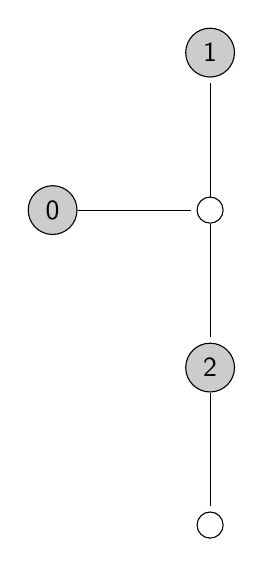
\begin{tikzpicture}[shorten >=2pt,auto, node distance=1cm,
		node_style/.style={circle,draw=black,fill=black!20!,font=\sffamily},
		node_style1/.style={circle,draw=black,fill=white!20!,font=\sffamily},
		edge_style/.style={draw=black}]
		
		\node[node_style] (n0) at (0,0)  {0};
		\node[node_style1] (n1) at (2,0)  {};
		\node[node_style] (n2) at (2,2)  {1};
		\node[node_style] (n3) at (2,-2)  {2};
		\node[node_style1] (n4) at (2,-4)  { };
		
		\draw[edge_style]  (n0) edge node{} (n1);
    	\draw[edge_style]  (n1) edge node{} (n2);
    	\draw[edge_style]  (n1) edge node{} (n3);
    	\draw[edge_style]  (n3) edge node{} (n4);

		\end{tikzpicture}}
\qquad
		\qquad
		\qquad
		\qquad 
\resizebox {0.2\textwidth} {0.5\height} {
		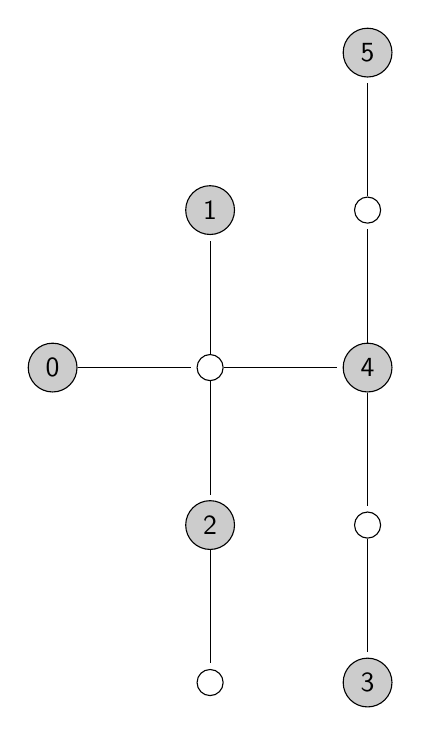
\begin{tikzpicture}[shorten >=2pt, auto, node distance=1cm,
		node_style1/.style={circle,draw=black,fill=white!20!,font=\sffamily},
		node_style/.style={circle,draw=black,fill=black!20!,font=\sffamily},
		edge_style/.style={draw=black}]
		
		\node[node_style] (n0) at (0,0)  {0};
		\node[node_style1] (n1) at (2,0)  {};
		\node[node_style] (n2) at (4,0)  {4};
		\node[node_style] (n3) at (2,2)  {1};
		\node[node_style1] (n4) at (4,2)  {};
		\node[node_style] (n5) at (4,4)  {5};
	    \node[node_style] (n6) at (2,-2)  {2};
		\node[node_style1] (n7) at (4,-2)  {};
		\node[node_style1] (n8) at (2,-4)  {};
		\node[node_style] (n9) at (4,-4)  {3};
		
		\draw[edge_style]  (n0) edge node{} (n1);
    	\draw[edge_style]  (n1) edge node{} (n2);
    	\draw[edge_style]  (n1) edge node{} (n3);
    	\draw[edge_style]  (n2) edge node{} (n4);
    	\draw[edge_style]  (n4) edge node{} (n5);
    	\draw[edge_style]  (n1) edge node{} (n6);
    	\draw[edge_style]  (n2) edge node{} (n7);
    	\draw[edge_style]  (n6) edge node{} (n8);
    	\draw[edge_style]  (n7) edge node{} (n9);
    
		\end{tikzpicture}}
			\qquad
		\qquad
		\qquad
\resizebox {0.3\textwidth} {0.6\height} {
		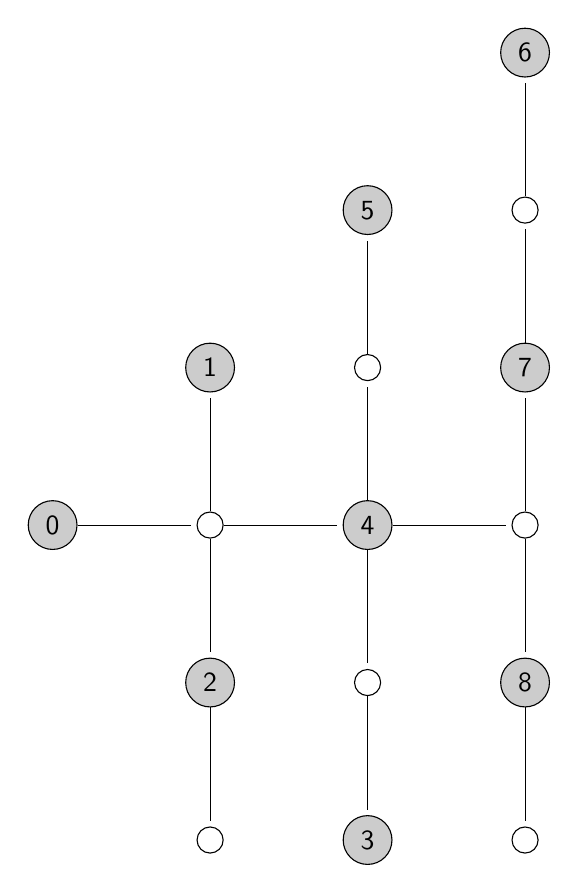
\begin{tikzpicture}[shorten >=2pt, auto, node distance=1cm,
		node_style1/.style={circle,draw=black,fill=white!!,font=\sffamily},
		node_style/.style={circle,draw=black,fill=black!20!,font=\sffamily},
		edge_style/.style={draw=black}]
		
		\node[node_style] (n0) at (0,0)  {0};
		\node[node_style1] (n1) at (2,0)  {};
		\node[node_style] (n2) at (4,0)  {4};
		\node[node_style1] (n3) at (6,0)  {};
		\node[node_style] (n4) at (2,2)  {1};
		\node[node_style1] (n5) at (4,2)  {};
	    \node[node_style] (n6) at (4,4)  {5};
		\node[node_style] (n7) at (6,2)  {7};
		\node[node_style1] (n8) at (6,4)  {};
		\node[node_style] (n9) at (6,6)  {6};
		\node[node_style] (n10) at (2,-2)  {2};
		\node[node_style1] (n11) at (2,-4)  {};
	    \node[node_style1] (n12) at (4,-2)  {};
		\node[node_style] (n13) at (4,-4)  {3};
		\node[node_style] (n14) at (6,-2)  {8};
		\node[node_style1] (n15) at (6,-4)  {};
		
		\draw[edge_style]  (n0) edge node{} (n1);
    	\draw[edge_style]  (n1) edge node{} (n2);
    	\draw[edge_style]  (n2) edge node{} (n3);
    	\draw[edge_style]  (n1) edge node{} (n4);
    	\draw[edge_style]  (n2) edge node{} (n5);
    	\draw[edge_style]  (n5) edge node{} (n6);
    	\draw[edge_style]  (n3) edge node{} (n7);
    	\draw[edge_style]  (n7) edge node{} (n8);
    	\draw[edge_style]  (n8) edge node{} (n9);
    	\draw[edge_style]  (n1) edge node{} (n10);
    	\draw[edge_style]  (n10) edge node{} (n11);
    	\draw[edge_style]  (n2) edge node{} (n12);
    	\draw[edge_style]  (n12) edge node{} (n13);
    	\draw[edge_style]  (n3) edge node{} (n14);
    	\draw[edge_style]  (n14) edge node{} (n15);
    	
		\end{tikzpicture}}\\

		\qquad $F_1(2)$
		\qquad \qquad \qquad \qquad \qquad \qquad 
		$F_2(2)$
		\qquad \qquad \qquad \qquad \qquad \qquad  \qquad \qquad 
		$F_3(2)$\\
\begin{center}
	\resizebox {0.45\textwidth} {0.7\height} {
		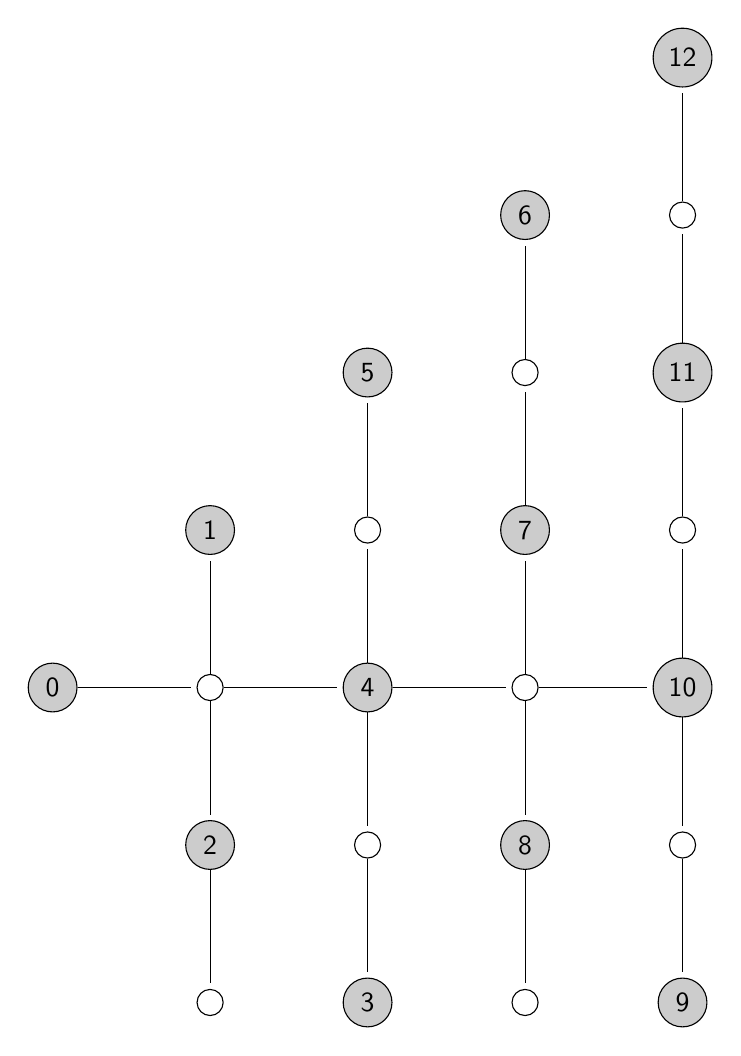
\begin{tikzpicture}[shorten >=2pt, auto, node distance=1cm,
		node_style1/.style={circle,draw=black,fill=white!20!,font=\sffamily},
		node_style/.style={circle,draw=black,fill=black!20!,font=\sffamily},
		edge_style/.style={draw=black}]
		
		\node[node_style] (n0) at (0,0)  {0};
		\node[node_style1] (n1) at (2,0)  {};
		\node[node_style] (n2) at (4,0)  {4};
		\node[node_style1] (n3) at (6,0)  {};
		\node[node_style] (n4) at (8,0)  {10};
		\node[node_style] (n5) at (2,2)  {1};
	    \node[node_style1] (n6) at (4,2)  {};
		\node[node_style] (n7) at (4,4)  {5};
		\node[node_style] (n8) at (6,2)  {7};
		\node[node_style1] (n9) at (6,4)  {};
		\node[node_style] (n10) at (6,6)  {6};
		\node[node_style1] (n11) at (8,2)  {};
	    \node[node_style] (n12) at (8,4)  {11};
		\node[node_style1] (n13) at (8,6)  {};
		\node[node_style] (n14) at (8,8)  {12};
		\node[node_style] (n15) at (2,-2)  {2};
		\node[node_style1] (n16) at (2,-4)  {};
		\node[node_style1] (n17) at (4,-2)  {};
		\node[node_style] (n18) at (4,-4)  {3};
		\node[node_style] (n19) at (6,-2)  {8};
	    \node[node_style1] (n20) at (6,-4)  {};
		\node[node_style1] (n21) at (8,-2)  {};
		\node[node_style] (n22) at (8,-4)  {9};

		\draw[edge_style]  (n0) edge node{} (n1);
    	\draw[edge_style]  (n1) edge node{} (n2);
    	\draw[edge_style]  (n2) edge node{} (n3);
    	\draw[edge_style]  (n3) edge node{} (n4);
    	\draw[edge_style]  (n1) edge node{} (n5);
    	\draw[edge_style]  (n2) edge node{} (n6);
    	\draw[edge_style]  (n6) edge node{} (n7);
    	\draw[edge_style]  (n3) edge node{} (n8);
    	\draw[edge_style]  (n8) edge node{} (n9);
    	\draw[edge_style]  (n9) edge node{} (n10);
    	\draw[edge_style]  (n4) edge node{} (n11);
    	\draw[edge_style]  (n11) edge node{} (n12);
    	\draw[edge_style]  (n12) edge node{} (n13);
    	\draw[edge_style]  (n13) edge node{} (n14);
    	\draw[edge_style]  (n1) edge node{} (n15);
    	\draw[edge_style]  (n15) edge node{} (n16);
    	\draw[edge_style]  (n2) edge node{} (n17);
    	\draw[edge_style]  (n17) edge node{} (n18);
    	\draw[edge_style]  (n3) edge node{} (n19);
    	\draw[edge_style]  (n19) edge node{} (n20);
    	\draw[edge_style]  (n4) edge node{} (n21);
		\draw[edge_style]  (n21) edge node{} (n22);
		\end{tikzpicture}}\\
		\begin{center}
        $F_4(2)$
    \end{center}
\end{center}
 \begin{center}
	\resizebox {0.55\textwidth} {0.7\height} {
	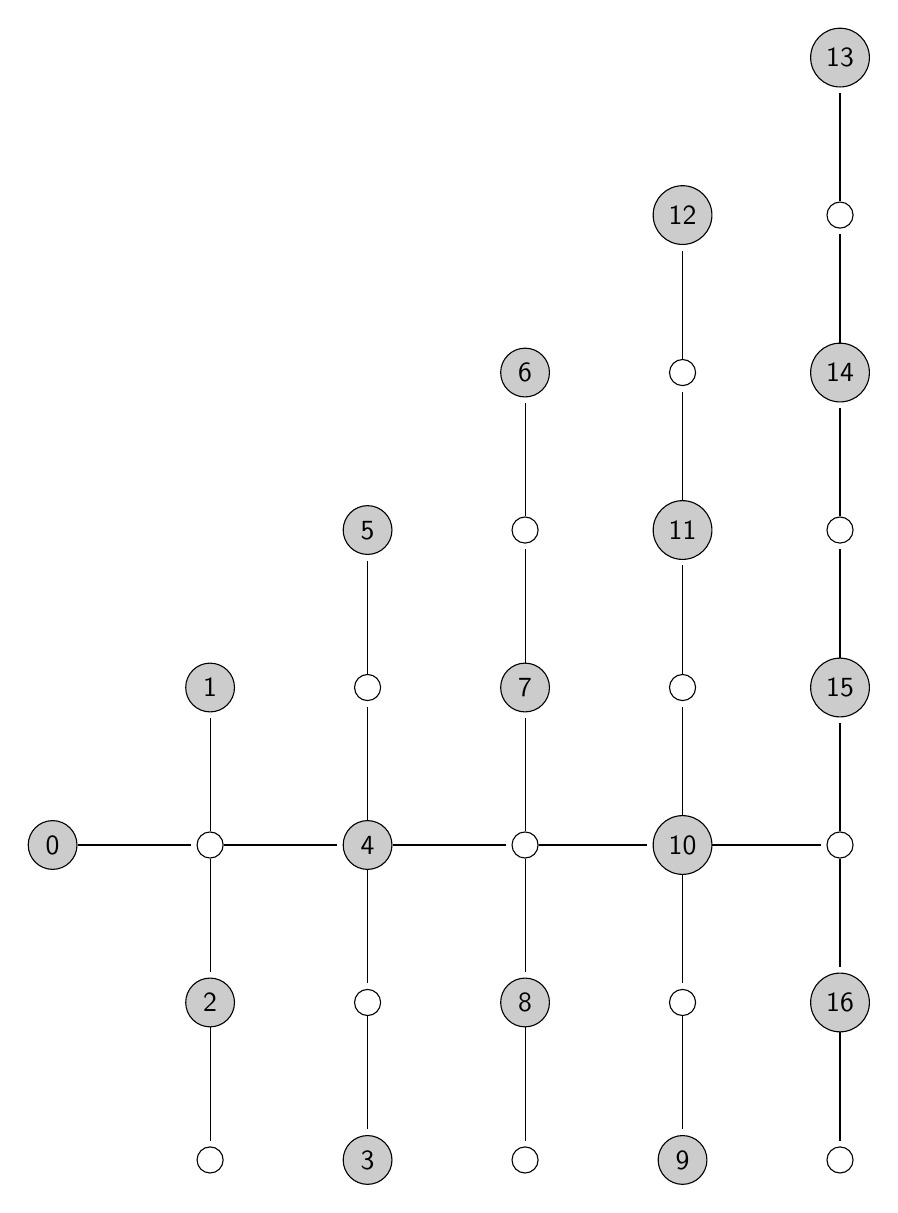
\begin{tikzpicture}[shorten >=2pt, auto, node distance=1cm,
		node_style1/.style={circle,draw=black,fill=white!20!,font=\sffamily},
		node_style/.style={circle,draw=black, fill=black!20!,font=\sffamily},
		edge_style/.style={draw=black}]
		
		\node[node_style] (n0) at (0,0)  {0};
		\node[node_style1] (n1) at (2,0)  {};
		\node[node_style] (n2) at (4,0)  {4};
		\node[node_style1] (n3) at (6,0)  {};
		\node[node_style] (n4) at (8,0)  {10};
		\node[node_style] (n5) at (2,2)  {1};
	    \node[node_style1] (n6) at (4,2)  {};
		\node[node_style] (n7) at (4,4)  {5};
		\node[node_style] (n8) at (6,2)  {7};
		\node[node_style1] (n9) at (6,4)  {};
		\node[node_style] (n10) at (6,6)  {6};
		\node[node_style1] (n11) at (8,2)  {};
	    \node[node_style] (n12) at (8,4)  {11};
		\node[node_style1] (n13) at (8,6)  {};
		\node[node_style] (n14) at (8,8)  {12};
		\node[node_style] (n15) at (2,-2)  {2};
		\node[node_style1] (n16) at (2,-4)  {};
		\node[node_style1] (n17) at (4,-2)  {};
		\node[node_style] (n18) at (4,-4)  {3};
		\node[node_style] (n19) at (6,-2)  {8};
	    \node[node_style1] (n20) at (6,-4)  {};
		\node[node_style1] (n21) at (8,-2)  {};
		\node[node_style] (n22) at (8,-4)  {9};
		\node[node_style1] (n23) at (10,0)  {};
		\node[node_style] (n24) at (10,2)  {15};
		\node[node_style1] (n25) at (10,4)  {};
		\node[node_style] (n26) at (10,6)  {14};
		\node[node_style1] (n27) at (10,8)  {};
	    \node[node_style] (n28) at (10,10)  {13};
		\node[node_style] (n29) at (10,-2)  {16};
		\node[node_style1] (n30) at (10,-4)  {};

		\draw[edge_style]  (n0) edge node{} (n1);
    	\draw[edge_style]  (n1) edge node{} (n2);
    	\draw[edge_style]  (n2) edge node{} (n3);
    	\draw[edge_style]  (n3) edge node{} (n4);
    	\draw[edge_style]  (n1) edge node{} (n5);
    	\draw[edge_style]  (n2) edge node{} (n6);
    	\draw[edge_style]  (n6) edge node{} (n7);
    	\draw[edge_style]  (n3) edge node{} (n8);
    	\draw[edge_style]  (n8) edge node{} (n9);
    	\draw[edge_style]  (n9) edge node{} (n10);
    	\draw[edge_style]  (n4) edge node{} (n11);
    	\draw[edge_style]  (n11) edge node{} (n12);
    	\draw[edge_style]  (n12) edge node{} (n13);
    	\draw[edge_style]  (n13) edge node{} (n14);
    	\draw[edge_style]  (n1) edge node{} (n15);
    	\draw[edge_style]  (n15) edge node{} (n16);
    	\draw[edge_style]  (n2) edge node{} (n17);
    	\draw[edge_style]  (n17) edge node{} (n18);
    	\draw[edge_style]  (n3) edge node{} (n19);
    	\draw[edge_style]  (n19) edge node{} (n20);
    	\draw[edge_style]  (n4) edge node{} (n21);
		\draw[edge_style]  (n21) edge node{} (n22);
		\draw[edge_style]  (n4) edge node{} (n23);
    	\draw[edge_style]  (n23) edge node{} (n24);
    	\draw[edge_style]  (n24) edge node{} (n25);
    	\draw[edge_style]  (n25) edge node{} (n26);
    	\draw[edge_style]  (n26) edge node{} (n27);
    	\draw[edge_style]  (n27) edge node{} (n28);
    	\draw[edge_style]  (n23) edge node{} (n29);
		\draw[edge_style]  (n29) edge node{} (n30);
		\end{tikzpicture}}\\
		\begin{center}
        $F_5(2)$ 
    \end{center}
\end{center}
\indent Then consider the vertices of the second color and continue the numbering until $v_1$ is reached and to which the integer \Big($\dfrac{(n+2)(n+3)}{2}-2$\Big) is assigned.\\
\resizebox {0.1\textwidth} {0.5\height} {
		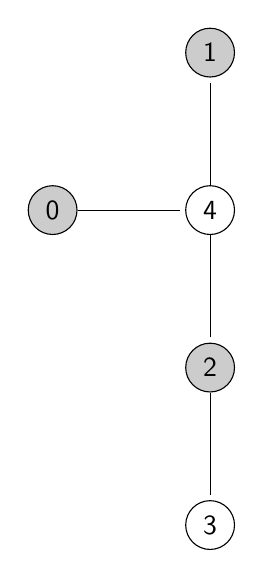
\begin{tikzpicture}[shorten >=2pt,auto, node distance=1cm,
		node_style/.style={circle,draw=black,fill=black!20!,font=\sffamily},
		node_style1/.style={circle,draw=black,fill=white!20!,font=\sffamily},
		edge_style/.style={draw=black}]
		
		\node[node_style] (n0) at (0,0)  {0};
		\node[node_style1] (n1) at (2,0)  {4};
		\node[node_style] (n2) at (2,2)  {1};
		\node[node_style] (n3) at (2,-2)  {2};
		\node[node_style1] (n4) at (2,-4)  {3};
		
		\draw[edge_style]  (n0) edge node{} (n1);
    	\draw[edge_style]  (n1) edge node{} (n2);
    	\draw[edge_style]  (n1) edge node{} (n3);
    	\draw[edge_style]  (n3) edge node{} (n4);

		\end{tikzpicture}}
\qquad
		\qquad
		\qquad
		\qquad 
\resizebox {0.2\textwidth} {0.5\height} {
		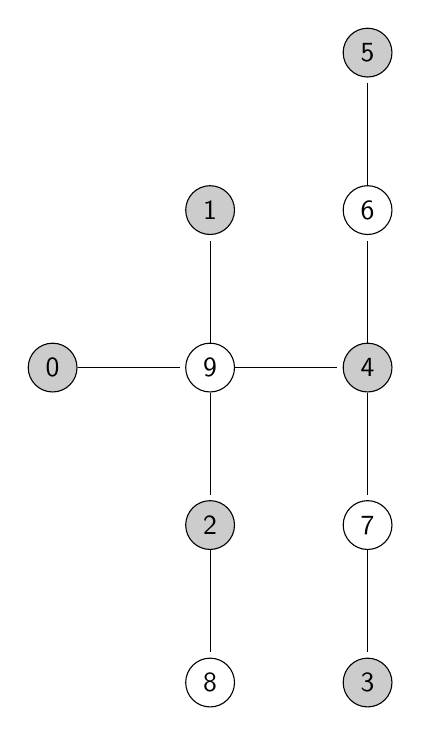
\begin{tikzpicture}[shorten >=2pt, auto, node distance=1cm,
		node_style1/.style={circle,draw=black,fill=white!20!,font=\sffamily},
		node_style/.style={circle,draw=black,fill=black!20!,font=\sffamily},
		edge_style/.style={draw=black}]
		
		\node[node_style] (n0) at (0,0)  {0};
		\node[node_style1] (n1) at (2,0)  {9};
		\node[node_style] (n2) at (4,0)  {4};
		\node[node_style] (n3) at (2,2)  {1};
		\node[node_style1] (n4) at (4,2)  {6};
		\node[node_style] (n5) at (4,4)  {5};
	    \node[node_style] (n6) at (2,-2)  {2};
		\node[node_style1] (n7) at (4,-2)  {7};
		\node[node_style1] (n8) at (2,-4)  {8};
		\node[node_style] (n9) at (4,-4)  {3};
		
		\draw[edge_style]  (n0) edge node{} (n1);
    	\draw[edge_style]  (n1) edge node{} (n2);
    	\draw[edge_style]  (n1) edge node{} (n3);
    	\draw[edge_style]  (n2) edge node{} (n4);
    	\draw[edge_style]  (n4) edge node{} (n5);
    	\draw[edge_style]  (n1) edge node{} (n6);
    	\draw[edge_style]  (n2) edge node{} (n7);
    	\draw[edge_style]  (n6) edge node{} (n8);
    	\draw[edge_style]  (n7) edge node{} (n9);
    
		\end{tikzpicture}}
			\qquad
		\qquad
		\qquad
\resizebox {0.3\textwidth} {0.6\height} {
		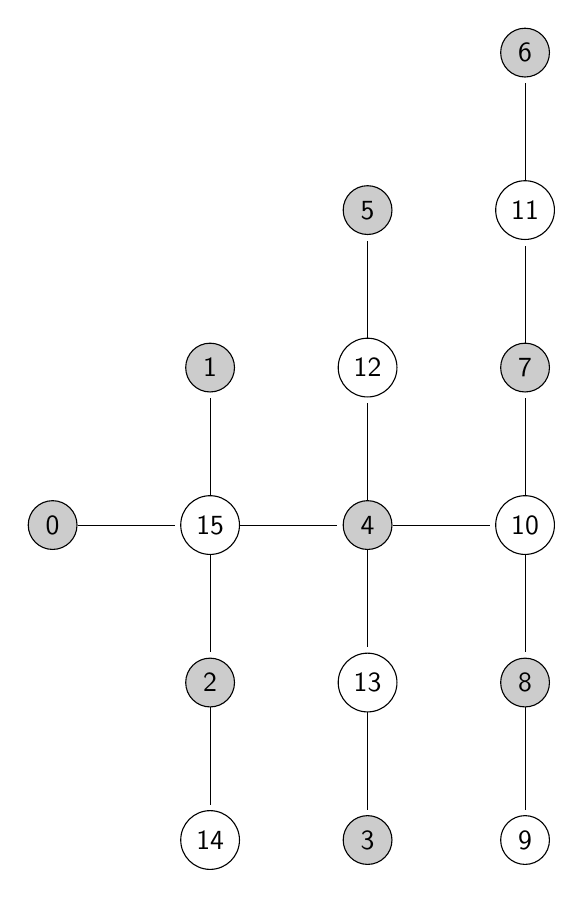
\begin{tikzpicture}[shorten >=2pt, auto, node distance=1cm,
		node_style1/.style={circle,draw=black,fill=white!!,font=\sffamily},
		node_style/.style={circle,draw=black,fill=black!20!,font=\sffamily},
		edge_style/.style={draw=black}]
		
		\node[node_style] (n0) at (0,0)  {0};
		\node[node_style1] (n1) at (2,0)  {15};
		\node[node_style] (n2) at (4,0)  {4};
		\node[node_style1] (n3) at (6,0)  {10};
		\node[node_style] (n4) at (2,2)  {1};
		\node[node_style1] (n5) at (4,2)  {12};
	    \node[node_style] (n6) at (4,4)  {5};
		\node[node_style] (n7) at (6,2)  {7};
		\node[node_style1] (n8) at (6,4)  {11};
		\node[node_style] (n9) at (6,6)  {6};
		\node[node_style] (n10) at (2,-2)  {2};
		\node[node_style1] (n11) at (2,-4)  {14};
	    \node[node_style1] (n12) at (4,-2)  {13};
		\node[node_style] (n13) at (4,-4)  {3};
		\node[node_style] (n14) at (6,-2)  {8};
		\node[node_style1] (n15) at (6,-4)  {9};
		
		\draw[edge_style]  (n0) edge node{} (n1);
    	\draw[edge_style]  (n1) edge node{} (n2);
    	\draw[edge_style]  (n2) edge node{} (n3);
    	\draw[edge_style]  (n1) edge node{} (n4);
    	\draw[edge_style]  (n2) edge node{} (n5);
    	\draw[edge_style]  (n5) edge node{} (n6);
    	\draw[edge_style]  (n3) edge node{} (n7);
    	\draw[edge_style]  (n7) edge node{} (n8);
    	\draw[edge_style]  (n8) edge node{} (n9);
    	\draw[edge_style]  (n1) edge node{} (n10);
    	\draw[edge_style]  (n10) edge node{} (n11);
    	\draw[edge_style]  (n2) edge node{} (n12);
    	\draw[edge_style]  (n12) edge node{} (n13);
    	\draw[edge_style]  (n3) edge node{} (n14);
    	\draw[edge_style]  (n14) edge node{} (n15);
    	
		\end{tikzpicture}}\\

		\qquad $F_1(2)$
		\qquad \qquad \qquad \qquad \qquad \qquad 
		$F_2(2)$
		\qquad \qquad \qquad \qquad \qquad \qquad  \qquad \qquad 
		$F_3(2)$\\
\begin{center}
	\resizebox {0.45\textwidth} {0.7\height} {
		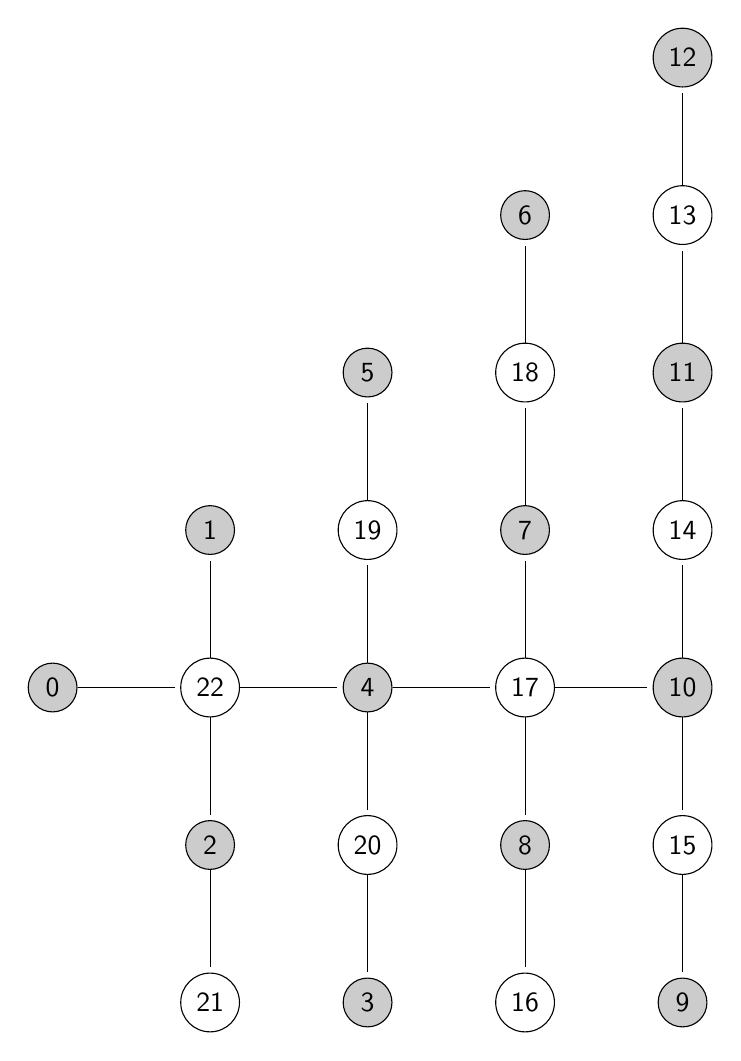
\begin{tikzpicture}[shorten >=2pt, auto, node distance=1cm,
		node_style1/.style={circle,draw=black,fill=white!20!,font=\sffamily},
		node_style/.style={circle,draw=black,fill=black!20!,font=\sffamily},
		edge_style/.style={draw=black}]
		
	    \node[node_style] (n0) at (0,0)  {0};
		\node[node_style1] (n1) at (2,0)  {22};
		\node[node_style] (n2) at (4,0)  {4};
		\node[node_style1] (n3) at (6,0)  {17};
		\node[node_style] (n4) at (8,0)  {10};
		\node[node_style] (n5) at (2,2)  {1};
	    \node[node_style1] (n6) at (4,2)  {19};
		\node[node_style] (n7) at (4,4)  {5};
		\node[node_style] (n8) at (6,2)  {7};
		\node[node_style1] (n9) at (6,4)  {18};
		\node[node_style] (n10) at (6,6)  {6};
		\node[node_style1] (n11) at (8,2)  {14};
	    \node[node_style] (n12) at (8,4)  {11};
		\node[node_style1] (n13) at (8,6)  {13};
		\node[node_style] (n14) at (8,8)  {12};
		\node[node_style] (n15) at (2,-2)  {2};
		\node[node_style1] (n16) at (2,-4)  {21};
		\node[node_style1] (n17) at (4,-2)  {20};
		\node[node_style] (n18) at (4,-4)  {3};
		\node[node_style] (n19) at (6,-2)  {8};
	    \node[node_style1] (n20) at (6,-4)  {16};
		\node[node_style1] (n21) at (8,-2)  {15};
		\node[node_style] (n22) at (8,-4)  {9};

		\draw[edge_style]  (n0) edge node{} (n1);
    	\draw[edge_style]  (n1) edge node{} (n2);
    	\draw[edge_style]  (n2) edge node{} (n3);
    	\draw[edge_style]  (n3) edge node{} (n4);
    	\draw[edge_style]  (n1) edge node{} (n5);
    	\draw[edge_style]  (n2) edge node{} (n6);
    	\draw[edge_style]  (n6) edge node{} (n7);
    	\draw[edge_style]  (n3) edge node{} (n8);
    	\draw[edge_style]  (n8) edge node{} (n9);
    	\draw[edge_style]  (n9) edge node{} (n10);
    	\draw[edge_style]  (n4) edge node{} (n11);
    	\draw[edge_style]  (n11) edge node{} (n12);
    	\draw[edge_style]  (n12) edge node{} (n13);
    	\draw[edge_style]  (n13) edge node{} (n14);
    	\draw[edge_style]  (n1) edge node{} (n15);
    	\draw[edge_style]  (n15) edge node{} (n16);
    	\draw[edge_style]  (n2) edge node{} (n17);
    	\draw[edge_style]  (n17) edge node{} (n18);
    	\draw[edge_style]  (n3) edge node{} (n19);
    	\draw[edge_style]  (n19) edge node{} (n20);
    	\draw[edge_style]  (n4) edge node{} (n21);
		\draw[edge_style]  (n21) edge node{} (n22);
		\end{tikzpicture}}\\
		\begin{center}
        $F_4(2)$
    \end{center}
\end{center}
 \begin{center}
	\resizebox {0.55\textwidth} {0.7\height} {
	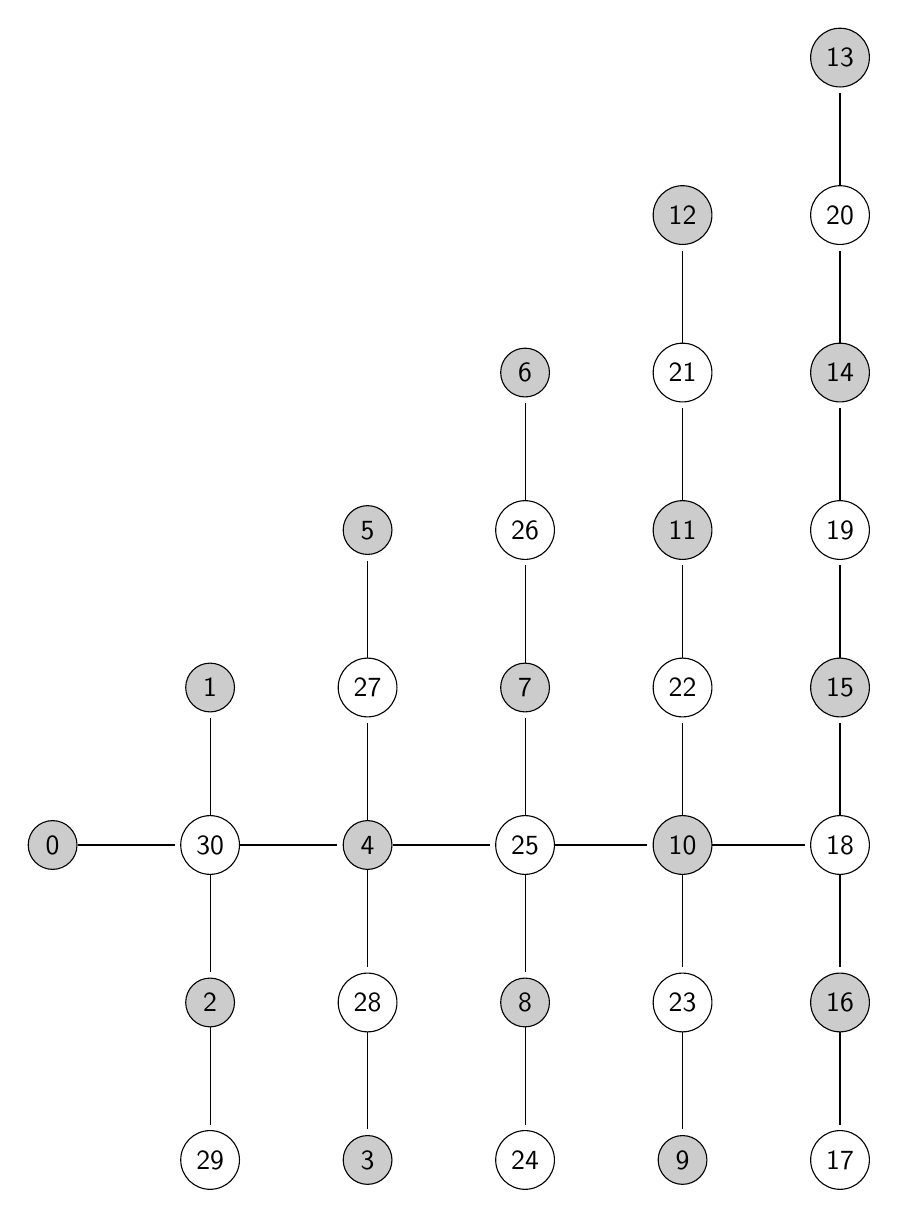
\begin{tikzpicture}[shorten >=2pt, auto, node distance=1cm,
		node_style1/.style={circle,draw=black,fill=white!20!,font=\sffamily},
		node_style/.style={circle,draw=black, fill=black!20!,font=\sffamily},
		edge_style/.style={draw=black}]
		
		\node[node_style] (n0) at (0,0)  {0};
		\node[node_style1] (n1) at (2,0)  {30};
		\node[node_style] (n2) at (4,0)  {4};
		\node[node_style1] (n3) at (6,0)  {25};
		\node[node_style] (n4) at (8,0)  {10};
		\node[node_style] (n5) at (2,2)  {1};
	    \node[node_style1] (n6) at (4,2)  {27};
		\node[node_style] (n7) at (4,4)  {5};
		\node[node_style] (n8) at (6,2)  {7};
		\node[node_style1] (n9) at (6,4)  {26};
		\node[node_style] (n10) at (6,6)  {6};
		\node[node_style1] (n11) at (8,2)  {22};
	    \node[node_style] (n12) at (8,4)  {11};
		\node[node_style1] (n13) at (8,6)  {21};
		\node[node_style] (n14) at (8,8)  {12};
		\node[node_style] (n15) at (2,-2)  {2};
		\node[node_style1] (n16) at (2,-4)  {29};
		\node[node_style1] (n17) at (4,-2)  {28};
		\node[node_style] (n18) at (4,-4)  {3};
		\node[node_style] (n19) at (6,-2)  {8};
	    \node[node_style1] (n20) at (6,-4)  {24};
		\node[node_style1] (n21) at (8,-2)  {23};
		\node[node_style] (n22) at (8,-4)  {9};
		\node[node_style1] (n23) at (10,0)  {18};
		\node[node_style] (n24) at (10,2)  {15};
		\node[node_style1] (n25) at (10,4)  {19};
		\node[node_style] (n26) at (10,6)  {14};
		\node[node_style1] (n27) at (10,8)  {20};
	    \node[node_style] (n28) at (10,10)  {13};
		\node[node_style] (n29) at (10,-2)  {16};
		\node[node_style1] (n30) at (10,-4)  {17};

		\draw[edge_style]  (n0) edge node{} (n1);
    	\draw[edge_style]  (n1) edge node{} (n2);
    	\draw[edge_style]  (n2) edge node{} (n3);
    	\draw[edge_style]  (n3) edge node{} (n4);
    	\draw[edge_style]  (n1) edge node{} (n5);
    	\draw[edge_style]  (n2) edge node{} (n6);
    	\draw[edge_style]  (n6) edge node{} (n7);
    	\draw[edge_style]  (n3) edge node{} (n8);
    	\draw[edge_style]  (n8) edge node{} (n9);
    	\draw[edge_style]  (n9) edge node{} (n10);
    	\draw[edge_style]  (n4) edge node{} (n11);
    	\draw[edge_style]  (n11) edge node{} (n12);
    	\draw[edge_style]  (n12) edge node{} (n13);
    	\draw[edge_style]  (n13) edge node{} (n14);
    	\draw[edge_style]  (n1) edge node{} (n15);
    	\draw[edge_style]  (n15) edge node{} (n16);
    	\draw[edge_style]  (n2) edge node{} (n17);
    	\draw[edge_style]  (n17) edge node{} (n18);
    	\draw[edge_style]  (n3) edge node{} (n19);
    	\draw[edge_style]  (n19) edge node{} (n20);
    	\draw[edge_style]  (n4) edge node{} (n21);
		\draw[edge_style]  (n21) edge node{} (n22);
		\draw[edge_style]  (n4) edge node{} (n23);
    	\draw[edge_style]  (n23) edge node{} (n24);
    	\draw[edge_style]  (n24) edge node{} (n25);
    	\draw[edge_style]  (n25) edge node{} (n26);
    	\draw[edge_style]  (n26) edge node{} (n27);
    	\draw[edge_style]  (n27) edge node{} (n28);
    	\draw[edge_style]  (n23) edge node{} (n29);
		\draw[edge_style]  (n29) edge node{} (n30);
		\end{tikzpicture}}\\
		\begin{center}
        $F_5(2)$ 
    \end{center}
\end{center}
		\newpage
\indent With the numbering scheme above, we generated the edge weights $1,2,3,\dots,\Big($\dfrac{(n+2)(n+3)}{2}-2$\Big)$.\\
\resizebox {0.1\textwidth} {0.5\height} {
		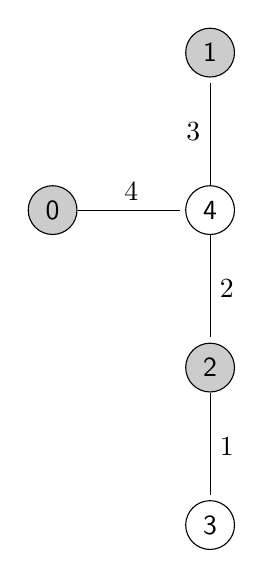
\begin{tikzpicture}[shorten >=2pt,auto, node distance=1cm,
		node_style/.style={circle,draw=black,fill=black!20!,font=\sffamily},
		node_style1/.style={circle,draw=black,fill=white!20!,font=\sffamily},
		edge_style/.style={draw=black}]
		
		\node[node_style] (n0) at (0,0)  {0};
		\node[node_style1] (n1) at (2,0)  {4};
		\node[node_style] (n2) at (2,2)  {1};
		\node[node_style] (n3) at (2,-2)  {2};
		\node[node_style1] (n4) at (2,-4)  {3};
		
		\draw[edge_style]  (n0) edge node{4} (n1);
    	\draw[edge_style]  (n1) edge node{3} (n2);
    	\draw[edge_style]  (n1) edge node{2} (n3);
    	\draw[edge_style]  (n3) edge node{1} (n4);

		\end{tikzpicture}}
\qquad
		\qquad
		\qquad
		\qquad 
\resizebox {0.2\textwidth} {0.5\height} {
		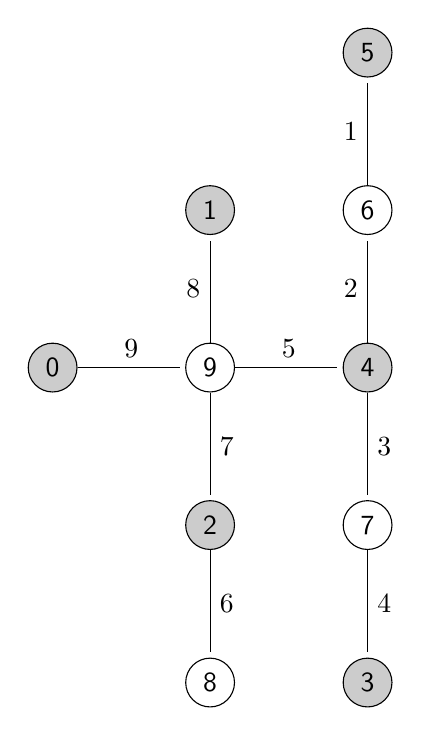
\begin{tikzpicture}[shorten >=2pt, auto, node distance=1cm,
		node_style1/.style={circle,draw=black,fill=white!20!,font=\sffamily},
		node_style/.style={circle,draw=black,fill=black!20!,font=\sffamily},
		edge_style/.style={draw=black}]
		
		\node[node_style] (n0) at (0,0)  {0};
		\node[node_style1] (n1) at (2,0)  {9};
		\node[node_style] (n2) at (4,0)  {4};
		\node[node_style] (n3) at (2,2)  {1};
		\node[node_style1] (n4) at (4,2)  {6};
		\node[node_style] (n5) at (4,4)  {5};
	    \node[node_style] (n6) at (2,-2)  {2};
		\node[node_style1] (n7) at (4,-2)  {7};
		\node[node_style1] (n8) at (2,-4)  {8};
		\node[node_style] (n9) at (4,-4)  {3};
		
		\draw[edge_style]  (n0) edge node{9} (n1);
    	\draw[edge_style]  (n1) edge node{5} (n2);
    	\draw[edge_style]  (n1) edge node{8} (n3);
    	\draw[edge_style]  (n2) edge node{2} (n4);
    	\draw[edge_style]  (n4) edge node{1} (n5);
    	\draw[edge_style]  (n1) edge node{7} (n6);
    	\draw[edge_style]  (n2) edge node{3} (n7);
    	\draw[edge_style]  (n6) edge node{6} (n8);
    	\draw[edge_style]  (n7) edge node{4} (n9);
    
		\end{tikzpicture}}
			\qquad
		\qquad
		\qquad
\resizebox {0.3\textwidth} {0.6\height} {
		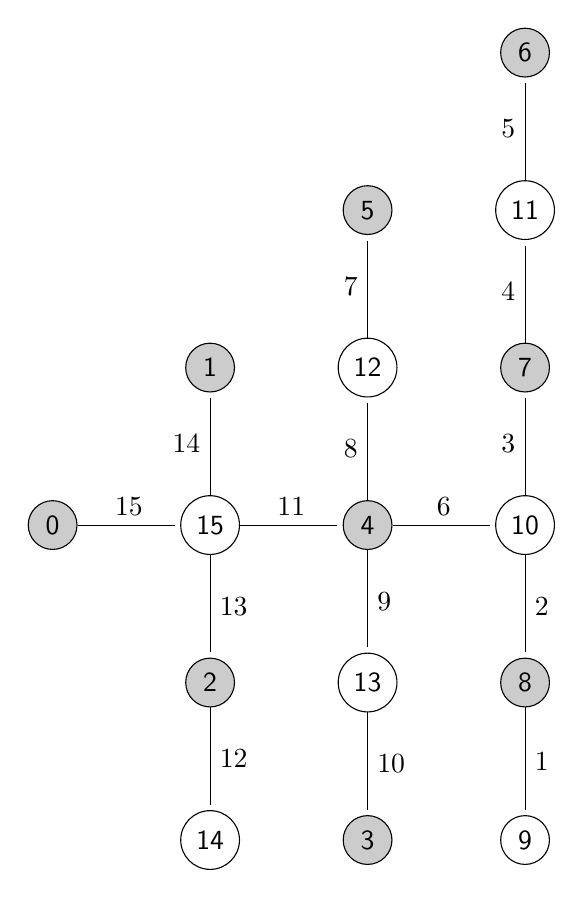
\begin{tikzpicture}[shorten >=2pt, auto, node distance=1cm,
		node_style1/.style={circle,draw=black,fill=white!!,font=\sffamily},
		node_style/.style={circle,draw=black,fill=black!20!,font=\sffamily},
		edge_style/.style={draw=black}]
		
		\node[node_style] (n0) at (0,0)  {0};
		\node[node_style1] (n1) at (2,0)  {15};
		\node[node_style] (n2) at (4,0)  {4};
		\node[node_style1] (n3) at (6,0)  {10};
		\node[node_style] (n4) at (2,2)  {1};
		\node[node_style1] (n5) at (4,2)  {12};
	    \node[node_style] (n6) at (4,4)  {5};
		\node[node_style] (n7) at (6,2)  {7};
		\node[node_style1] (n8) at (6,4)  {11};
		\node[node_style] (n9) at (6,6)  {6};
		\node[node_style] (n10) at (2,-2)  {2};
		\node[node_style1] (n11) at (2,-4)  {14};
	    \node[node_style1] (n12) at (4,-2)  {13};
		\node[node_style] (n13) at (4,-4)  {3};
		\node[node_style] (n14) at (6,-2)  {8};
		\node[node_style1] (n15) at (6,-4)  {9};
		
		\draw[edge_style]  (n0) edge node{15} (n1);
    	\draw[edge_style]  (n1) edge node{11} (n2);
    	\draw[edge_style]  (n2) edge node{6} (n3);
    	\draw[edge_style]  (n1) edge node{14} (n4);
    	\draw[edge_style]  (n2) edge node{8} (n5);
    	\draw[edge_style]  (n5) edge node{7} (n6);
    	\draw[edge_style]  (n3) edge node{3} (n7);
    	\draw[edge_style]  (n7) edge node{4} (n8);
    	\draw[edge_style]  (n8) edge node{5} (n9);
    	\draw[edge_style]  (n1) edge node{13} (n10);
    	\draw[edge_style]  (n10) edge node{12} (n11);
    	\draw[edge_style]  (n2) edge node{9} (n12);
    	\draw[edge_style]  (n12) edge node{10} (n13);
    	\draw[edge_style]  (n3) edge node{2} (n14);
    	\draw[edge_style]  (n14) edge node{1} (n15);
    	
		\end{tikzpicture}}\\

		\qquad $F_1(2)$
		\qquad \qquad \qquad \qquad \qquad \qquad 
		$F_2(2)$
		\qquad \qquad \qquad \qquad \qquad \qquad  \qquad \qquad 
		$F_3(2)$\\
		\\
\begin{center}
	\resizebox {0.45\textwidth} {0.7\height} {
		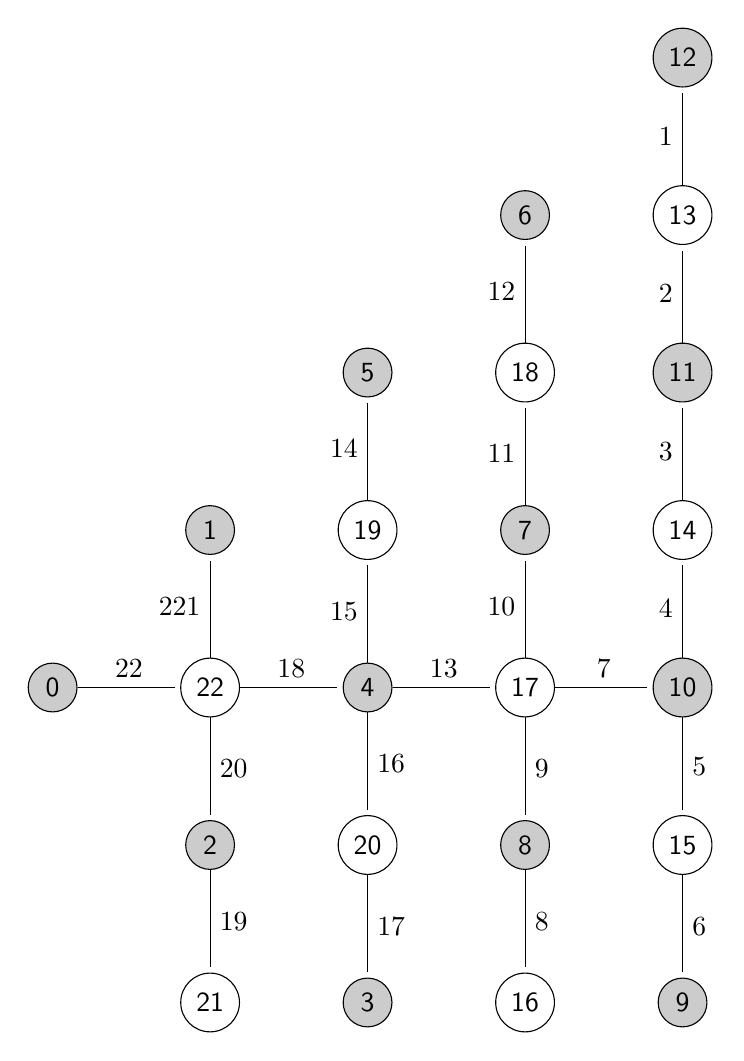
\begin{tikzpicture}[shorten >=2pt, auto, node distance=1cm,
		node_style1/.style={circle,draw=black,fill=white!20!,font=\sffamily},
		node_style/.style={circle,draw=black,fill=black!20!,font=\sffamily},
		edge_style/.style={draw=black}]
		
	\node[node_style] (n0) at (0,0)  {0};
		\node[node_style1] (n1) at (2,0)  {22};
		\node[node_style] (n2) at (4,0)  {4};
		\node[node_style1] (n3) at (6,0)  {17};
		\node[node_style] (n4) at (8,0)  {10};
		\node[node_style] (n5) at (2,2)  {1};
	    \node[node_style1] (n6) at (4,2)  {19};
		\node[node_style] (n7) at (4,4)  {5};
		\node[node_style] (n8) at (6,2)  {7};
		\node[node_style1] (n9) at (6,4)  {18};
		\node[node_style] (n10) at (6,6)  {6};
		\node[node_style1] (n11) at (8,2)  {14};
	    \node[node_style] (n12) at (8,4)  {11};
		\node[node_style1] (n13) at (8,6)  {13};
		\node[node_style] (n14) at (8,8)  {12};
		\node[node_style] (n15) at (2,-2)  {2};
		\node[node_style1] (n16) at (2,-4)  {21};
		\node[node_style1] (n17) at (4,-2)  {20};
		\node[node_style] (n18) at (4,-4)  {3};
		\node[node_style] (n19) at (6,-2)  {8};
	    \node[node_style1] (n20) at (6,-4)  {16};
		\node[node_style1] (n21) at (8,-2)  {15};
		\node[node_style] (n22) at (8,-4)  {9};
		
	    \draw[edge_style]  (n0) edge node{22} (n1);
    	\draw[edge_style]  (n1) edge node{18} (n2);
    	\draw[edge_style]  (n2) edge node{13} (n3);
    	\draw[edge_style]  (n3) edge node{7} (n4);
    	\draw[edge_style]  (n1) edge node{221} (n5);
    	\draw[edge_style]  (n2) edge node{15} (n6);
    	\draw[edge_style]  (n6) edge node{14} (n7);
    	\draw[edge_style]  (n3) edge node{10} (n8);
    	\draw[edge_style]  (n8) edge node{11} (n9);
    	\draw[edge_style]  (n9) edge node{12} (n10);
    	\draw[edge_style]  (n4) edge node{4} (n11);
    	\draw[edge_style]  (n11) edge node{3} (n12);
    	\draw[edge_style]  (n12) edge node{2} (n13);
    	\draw[edge_style]  (n13) edge node{1} (n14);
    	\draw[edge_style]  (n1) edge node{20} (n15);
    	\draw[edge_style]  (n15) edge node{19} (n16);
    	\draw[edge_style]  (n2) edge node{16} (n17);
    	\draw[edge_style]  (n17) edge node{17} (n18);
    	\draw[edge_style]  (n3) edge node{9} (n19);
    	\draw[edge_style]  (n19) edge node{8} (n20);
    	\draw[edge_style]  (n4) edge node{5} (n21);
		\draw[edge_style]  (n21) edge node{6} (n22);
		\end{tikzpicture}}\\
		\begin{center}
        $F_4(2)$
    \end{center}
\end{center}
 \begin{center}
	\resizebox {0.55\textwidth} {0.7\height} {
	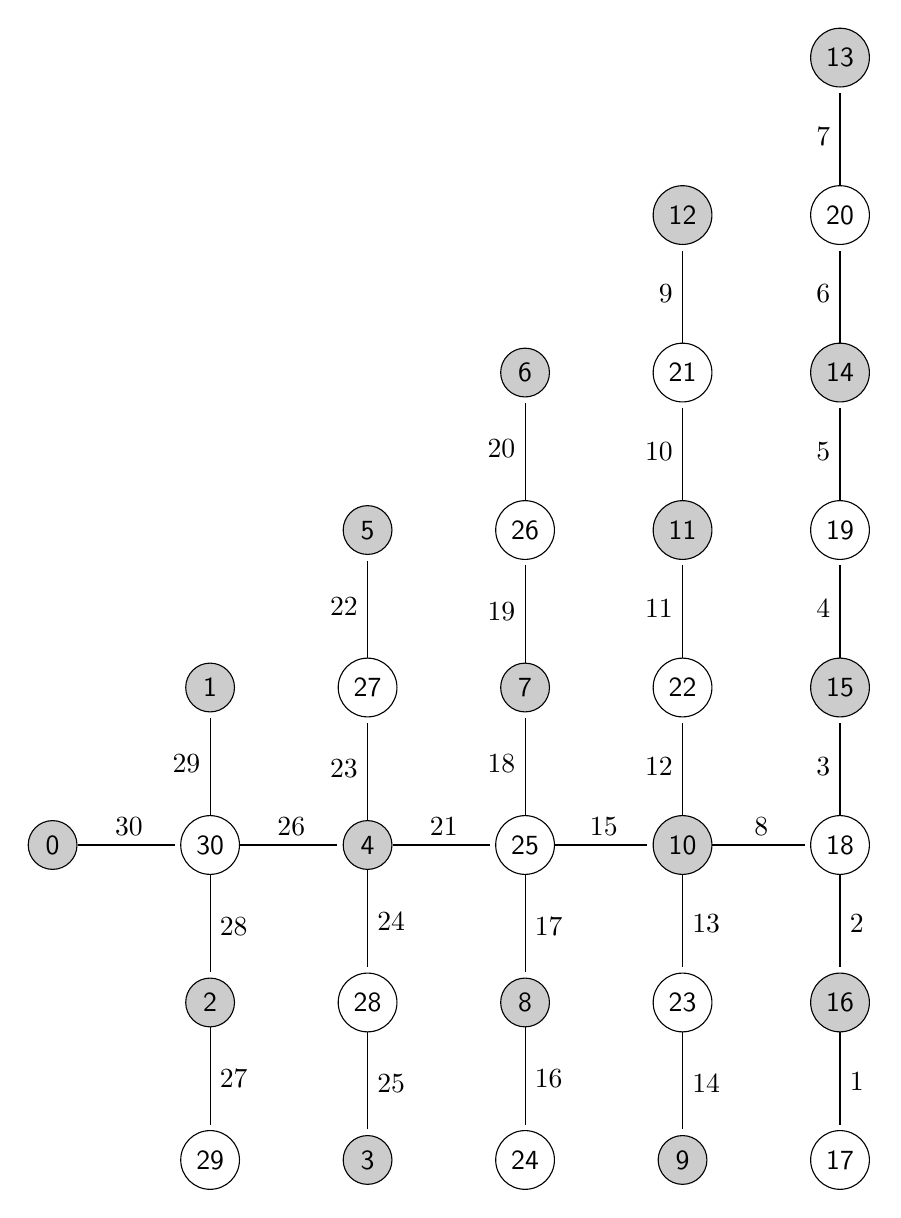
\begin{tikzpicture}[shorten >=2pt, auto, node distance=1cm,
		node_style1/.style={circle,draw=black,fill=white!20!,font=\sffamily},
		node_style/.style={circle,draw=black, fill=black!20!,font=\sffamily},
		edge_style/.style={draw=black}]
		
		\node[node_style] (n0) at (0,0)  {0};
		\node[node_style1] (n1) at (2,0)  {30};
		\node[node_style] (n2) at (4,0)  {4};
		\node[node_style1] (n3) at (6,0)  {25};
		\node[node_style] (n4) at (8,0)  {10};
		\node[node_style] (n5) at (2,2)  {1};
	    \node[node_style1] (n6) at (4,2)  {27};
		\node[node_style] (n7) at (4,4)  {5};
		\node[node_style] (n8) at (6,2)  {7};
		\node[node_style1] (n9) at (6,4)  {26};
		\node[node_style] (n10) at (6,6)  {6};
		\node[node_style1] (n11) at (8,2)  {22};
	    \node[node_style] (n12) at (8,4)  {11};
		\node[node_style1] (n13) at (8,6)  {21};
		\node[node_style] (n14) at (8,8)  {12};
		\node[node_style] (n15) at (2,-2)  {2};
		\node[node_style1] (n16) at (2,-4)  {29};
		\node[node_style1] (n17) at (4,-2)  {28};
		\node[node_style] (n18) at (4,-4)  {3};
		\node[node_style] (n19) at (6,-2)  {8};
	    \node[node_style1] (n20) at (6,-4)  {24};
		\node[node_style1] (n21) at (8,-2)  {23};
		\node[node_style] (n22) at (8,-4)  {9};
		\node[node_style1] (n23) at (10,0)  {18};
		\node[node_style] (n24) at (10,2)  {15};
		\node[node_style1] (n25) at (10,4)  {19};
		\node[node_style] (n26) at (10,6)  {14};
		\node[node_style1] (n27) at (10,8)  {20};
	    \node[node_style] (n28) at (10,10)  {13};
		\node[node_style] (n29) at (10,-2)  {16};
		\node[node_style1] (n30) at (10,-4)  {17};

		\draw[edge_style]  (n0) edge node{30} (n1);
    	\draw[edge_style]  (n1) edge node{26} (n2);
    	\draw[edge_style]  (n2) edge node{21} (n3);
    	\draw[edge_style]  (n3) edge node{15} (n4);
    	\draw[edge_style]  (n1) edge node{29} (n5);
    	\draw[edge_style]  (n2) edge node{23} (n6);
    	\draw[edge_style]  (n6) edge node{22} (n7);
    	\draw[edge_style]  (n3) edge node{18} (n8);
    	\draw[edge_style]  (n8) edge node{19} (n9);
    	\draw[edge_style]  (n9) edge node{20} (n10);
    	\draw[edge_style]  (n4) edge node{12} (n11);
    	\draw[edge_style]  (n11) edge node{11} (n12);
    	\draw[edge_style]  (n12) edge node{10} (n13);
    	\draw[edge_style]  (n13) edge node{9} (n14);
    	\draw[edge_style]  (n1) edge node{28} (n15);
    	\draw[edge_style]  (n15) edge node{27} (n16);
    	\draw[edge_style]  (n2) edge node{24} (n17);
    	\draw[edge_style]  (n17) edge node{25} (n18);
    	\draw[edge_style]  (n3) edge node{17} (n19);
    	\draw[edge_style]  (n19) edge node{16} (n20);
    	\draw[edge_style]  (n4) edge node{13} (n21);
		\draw[edge_style]  (n21) edge node{14} (n22);
		\draw[edge_style]  (n4) edge node{8} (n23);
    	\draw[edge_style]  (n23) edge node{3} (n24);
    	\draw[edge_style]  (n24) edge node{4} (n25);
    	\draw[edge_style]  (n25) edge node{5} (n26);
    	\draw[edge_style]  (n26) edge node{6} (n27);
    	\draw[edge_style]  (n27) edge node{7} (n28);
    	\draw[edge_style]  (n23) edge node{2} (n29);
		\draw[edge_style]  (n29) edge node{1} (n30);
		\end{tikzpicture}}\\
		\begin{center}
        $F_5(2)$ 
    \end{center}
\end{center}
\indent In general, this numbering scheme will continue for $n\in\mathbb{N}$ and will result in a new family of graceful trees which is the $F_n(2)$, $n\in \mathbb{N}$.
\section{Conclusion}
\indent
\indent A new family of graceful trees was shown graceful, the $F_n (2)$ trees, for all $n\in \mathbb{N}$. By trial-and-error, patterns and generalizations were observed in the first few members of the family. The next member of $F_{n+1} (2)$ is constructed by considering the $J_{n+2}$ tree with a parent path $P_{n+2}=v_0 v_1 v_2 \dots v_{n+1}$ and by planting a path $\overline{P}_2$ of length two to vertices $v_1$, $v_2$, \dots,  $v_{n+1}$.
\section{References}
\begin{thebibliography}{9}
	\bibitem{Loyola} Loyola, J.\emph{On Families and Generation of Graceful Trees}. Master's Thesis. (1991)
	\bibitem{Castilan and Zarraga}  Castilan, M.G. and Zarraga, N. \emph{Three New Families of Graceful Trees}. Special Problem. (2010)
\end{thebibliography}
\end{document}